\documentclass[12pt,a4paper,catalan]{article}
\usepackage[utf8]{inputenc}
\usepackage{graphicx} % for images
\usepackage{booktabs} % for tables
\usepackage{fancyhdr} % for header and footers
\usepackage{titlesec}
\usepackage{hyperref} % for links 
\usepackage{minted}
\usepackage{amsmath} % for math annotations
\usepackage{todonotes}
\usepackage{enumitem}
\usepackage{amsfonts}
\usepackage{subcaption}
\usepackage[catalan]{babel}
\usepackage{cite}
\usepackage{fancyref}
\usepackage{afterpage}
%\usepackage{caption}
%\usepackage{siunitx}


%Definició de noms:
\newcommand{\titleTFG}{Ciència de les dades aplicada a resultats acadèmics: perfil d'estudiants i predicció de notes}
\newcommand{\littletitleTFG}{Ciència de les dades aplicada a resultats acadèmics}
\newcommand{\myname}{Xavier Moreno Liceras}

\newcommand\blankpage{%
    \null
    \thispagestyle{empty}%
    \addtocounter{page}{-1}%
    \newpage}

\setlength{\parindent}{0pt}

%Definició de colors:
\definecolor{bgcode}{rgb}{0.93, 0.93, 0.93}

\setcounter{secnumdepth}{4}
\setcounter{tocdepth}{4}
\titleformat{\paragraph}
{\normalfont\normalsize\bfseries}{\theparagraph}{1em}{}
\titlespacing*{\paragraph}
{0pt}{3.25ex plus 1ex minus .2ex}{1.5ex plus .2ex}

% define letters
\makeatletter
\def\iddots{\mathinner{\mkern1mu\raise\p@
\vbox{\kern7\p@\hbox{.}}\mkern2mu
\raise4\p@\hbox{.}\mkern2mu\raise7\p@\hbox{.}\mkern1mu}}
\makeatother

\pagestyle{fancy}
\fancyhf{}
\rhead{\littletitleTFG}
\cfoot{\thepage}
 
\hypersetup{
    unicode=true,          % non-Latin characters in Acrobat’s bookmarks
    pdftitle={\titleTFG},    % title
    pdfsubject={TFG},
    pdfauthor={\myname},     % author
    pdfproducer={\LaTeX},   % producer
    pdfcreator={\myname},   % creator of the document
    pdfkeywords={tutor} {innovació docent} {predicció} {pla d'acció tutorial}, % list of keywords
    colorlinks=true,       % false: boxed links; true: colored links
    linkcolor=blue,          % color of internal links (change box color with linkbordercolor)
    citecolor=blue,        % color of links to bibliography
    urlcolor=blue           % color of external links
}

\begin{document}
\bibstyle{plain}
\thispagestyle{empty}

\begin{titlepage}
\begin{center}
\begin{figure}[h]
\begin{center}

\includegraphics[width=6cm]{img/ub.png}
\end{center}
\end{figure}

\textbf{\LARGE Treball final de grau} \\
\vspace*{.5cm}
\textbf{\LARGE GRAU D'ENGINYERIA INFORMÀTICA } \\
\vspace*{.5cm}
\textbf{\LARGE Facultat de Matemàtiques \\ Universitat de Barcelona} \\
\vspace*{1.5cm}
\rule{\textwidth}{0.1mm}\\
\begin{LARGE}
\textbf{\titleTFG} \\
\end{LARGE}
\rule{\textwidth}{0.1mm}\\

\vspace{1cm}

\begin{flushright}
\textbf{\LARGE Autor: \myname}

\vspace*{2cm}

\renewcommand{\arraystretch}{1.5}
\begin{tabular}{ll}
\textbf{\Large Directora:} & \textbf{\Large Laura Igual } \\
\textbf{\Large Realitzat a:} & \textbf{\Large  Departament   } \\
 & \textbf{\Large Matemàtica Aplicada y Anàlisi} \\
\\

\textbf{\Large Barcelona,} & \textbf{\Large \today }



\end{tabular}

\end{flushright}

\end{center}
\afterpage{\blankpage}
\end{titlepage}

\pagenumbering{roman}

\section*{\textit{Abstract}}
\textit{This paper is part of an innovative educational project. Its main aim is to provide a support system for teachers, designed to help them when creating any student's profile. In order to create this intelligent system for teachers, data from Mathematics Faculty has been retrieved and analysed. This analysis focuses on student's profiles and score predictions. The profile analysis is bases on previous years' grades as well as an average of how many students abandon their studies. On a side note, it develops also a score and grade prediction as well as a ranking of subjects, listed by level of difficulty depending on the student.}

\section*{\textit{Resum}}
\textit{Aquest treball està dins del marc d'un projecte d'innovació docent, en el que es proposa una eina de suport per al tutor d'estudis, la qual permeti ajudar al tutor a conèixer millor el perfil de cada alumne que tutoritza, realitzar el seguiment i aconsellar-lo. Per poder arribar a fer aquest sistema intel·ligent per al tutor d'estudis, s'ha realitzat un anàlisi basat en ciència de les dades sobre els resultats acadèmics de la Facultat de Matemàtiques. L'anàlisi es centra en l'exploració de perfils d'estudiants i en la predicció de notes. Dins l'anàlisi de perfils d'estudiants es mira la taxa d'abandonament per cada perfil i la relació que té cadascun respecte els perfils del curs anterior. Per altra banda, es realitza un sistema de predicció de notes i un rànquing d'assignatures ordenades per dificultat enfocat a l'alumne.}

\section*{\textit{Resumen}}
\textit{Este trabajo está dentro del marco de un proyecto de innovación docente, en el que se propone una herramienta de soporte para el tutor de estudios, la cual permita ayudar al tutor a conocer mejor el perfil de cada alumno que tutoriza. Para poder llegar a hacer este sistema inteligente para el tutor de estudios, se ha realizado un análisis basado en ciència de los datos sobre los resultados académicos de la Facultad de Matemáticas. El análisis se centra en la exploración de perfiles de estudiantes y en la predicción de cualificaciones. Dentro del análisis de perfiles de estudiantes se mira la tasa de abandono para cada perfil y la relación que tiene cada uno respecto a los perfiles del curso anterior. Por otro lado, se realiza un sistema de predicción de cualificaciones y un ránquing de asignaturas ordenadas por dificultad enfocada al alumno.}


\newpage 

\addto\captionsenglish{
  \renewcommand{\contentsname}%
    {Índex}%
}


{\hypersetup{linkcolor=black}
	\thispagestyle{empty}
	\tableofcontents
	\thispagestyle{empty}
}

\newpage

\pagenumbering{arabic} 
\setcounter{page}{1}


\section{Introducció}
Un dels components bàsics de l'activitat docent a la Universitat de Barcelona és l'acció tutorial, la qual té com a finalitat guiar i aconsellar a l'estudiant durant la seva etapa d'estudis. Ajuda a l'estudiant a millorar el seu rendiment, la seva orientació professional, i el més important, ajuda a prendre decissions que afavoreixin els seus resultats acadèmics i la seva satisfacció. El pla d'acció tutorial (PAT) en els graus de Matemàtiques i d'Enginyeria Informàtica a la Facultat de Matemàtiques realitza un conjunt ordenat d'accions sistemàtiques prèviament planificades. Una de les coses que impulsa el PAT és l'assignació d'un tutor d'estudis a un grup d'estudiants. Un tutor d'estudis té com a finalitat, entre altres, acompanyar a l'alumnat durant el seu transcurs a la universitat des de l'inici del grau, fins al final, donant consell cara al món professional.
\\
\\
Ens hem trobat amb el problema que un tutor d'estudis, al tutoritzar a un grup d'alumnes, no és capaç de contemplar detingudament cadascun d'aquests. Els pot guiar de forma genèrica, seguint el pla d'acció tutorial. S'ha pogut observar al llarg dels anys, per exemple, que alumnes amb qualificacions moderades a primer i segon del grau d'Enginyeria Informàtica tenen problemes per afrontar certes assignatures de tercer. Això s'ha pogut observar al llarg dels anys, però i si estem perdent altres problemes o fets importants que no s'han pogut obervar fins ara? És això el que volem explorar i fer conclusions que no s'hagin pogut arribar. Arran d'això, s'ha fet una petició al Vicerectorat de Política Docent per dur a terme un projecte que facilités el treball al tutor d'estudis. D'aquí neix un projecte d'innovació docent amb el títol: \textit{Sistema intel·ligent de suport per al tutor d'estudis}.
\\
\\
La finalitat del projecte d'innovació docent és la creació d'una eina que el tutor pugui consultar i li ajudi a prendre decissions cara a les seves tutories. Aquesta eina ha de permetre al tutor visualitzar la trajectòria d'un alumne, fer recomanacions específiques per cadascun d'ells, entre altres. Un dels recursos principals d'aquest projecte són les dades, ja que són les que ens permetran arribar a conclusions i poder construïr l'eina per al tutor d'estudis. Les dades han sigut obtingudes a través del Vicerectorat de Política Docent.
\\
\\
Aquest treball final de grau forma part del projecte d'innovació docent, i es centra en l'estudi estadístic de les dades dels resultats acadèmics de la Facultat de Matemàtiques de la UB. L'objectiu és desenvolupar la base per poder ampliar, en la següent fase del projecte, el sistema per al tutor d'estudis. En aquest treball ens hem centrat en l'exploració dels perfils d'estudiants dels primers cursos de cadascun dels graus impartits en la Facultat de Matemàtiques. També s'ha treballat en un sistema de predicció de notes d'un alumne cara a la seva pròxima matriculació. A més s'ha desenvolupat un rànquing de dificultat de notes d'assignatures no matriculades d'un alumne a partir d'un predictor de notes. L'objectiu general d'aquest treball és obtenir coneixement a partir de les dades, i és per això que hem enfocat aquest projecte com a un projecte de ciència de les dades.


\newpage


\section{Descripció del problema}
\subsection{Projecte d'innovació docent}
Aquest Treball de Fi de Grau, s'enmarca dins d'un projecte d'innovació docent \cite{pid} que va nèixer al Departament de Matemàtica Aplicada i Anàlisi (MAIA) i el Departament de Metòdes de Investigació i Diagnòstic en Educació (MIDE).
\\
\\
Com ja s'ha dit, la finalitat del projecte d'innovació docent és el desenvolupament d'un sistema intel·ligent de suport al tutor d'estudis, i per dur-lo a terme el projecte s'ha dividit en 5 fases.

\subparagraph{Fase 1}
Adquisició, ordenació, centralització i anonimització de les dades curriculars disponibles dels alumnes. La fase inicial on es deixen les dades preparades per poder treballar amb elles.

\subparagraph{Fase 2}
Anàlisi de les dades mitjançant tècniques de ciències de les dades. Fer un anàlisi estadístic de les dades que tenim i aplicar ciència de les dades per explorar la informació amagada darrere de les dades.

\subparagraph{Fase 3}
Anàlisi de les dades mitjançant tècniques d’aprenentatge automàtic. A partir de les dades aplicar algoritmes de predicció de dades per poder predir les notes d'un alumne en base a les seves notes i la de la resta d'alumnes.

\subparagraph{Fase 4}
Desenvolupament del sistema intel·ligent. En aquesta fase es busca el desenvolupament de l'eina de suport per al tutor d'estudis.

\subparagraph{Fase 5}
Avaluació. S'avalua el sistema per tal de fer proves i buscar mancances i errors del propi sistema.
\\
\\
Aquest treball forma part de la fase 1, 2 i 3. Les fases 4 i 5 són l'altre part del projecte, i no s'en parlarà en aquest treball.

\subsection{Ciència de les dades}
\label{subsec:cienciadelesdades}
La ciència de les dades és el conjunt d'etapes per tal d'arribar a un resultat, en forma de coneixement, a partir d'un conjunt de dades. Aquesta aplica un conjunt de tècniques de diferents àreas, com ara matemàtiques, estadística, teoria de la informació o tecnologia de l'extracció d'informació.
\\
\\
Un projecte de ciència de les dades es separa en diverses etapes:
\begin{enumerate}
	\item \textbf{Plantejament de preguntes} Què és el que volem explorar? Té sentit el que ens estem plantejant?
	\item \textbf{Adquisició de les dades} Com és la font d'obtenció de les dades? (Base de dades, \textit{Web Scraping}, fitxer .csv)
	\item \textbf{Descripció} Aquesta fase abasta tres processos
	\begin{enumerate}
		\item \textbf{Neteja de dades} Com hem de netejar i separar les dades? (mostres atípiques, filtració, redució de dimensions, normalització, extracció de característiques)
		\item \textbf{Agregació} Com hem de recol·lectar i resumir les dades? (promig, desviació estàndard, box plots)
		\item \textbf{Enriquiment} Com podem afegir més informació a les nostres dades? (Cerca a altres fonts de dades adicionals)
	\end{enumerate}
	\item \textbf{Descobriment} Podem segmentar les nostres dades per trobar grups naturals i disgregats? (Clusterització, visualització)
	\item \textbf{Anàlisi} Com hem de modelar les nostres dades? (Com estan de relacionades cada variable?, Com podem determinar quines són les variables importants?)
	\item \textbf{Predicció} A partir de les dades que tenim, què podem predir del futur? (Regressions, classificadors, recomanadors)
	\item \textbf{Avaluació} Com de segurs estem dels nostres resultats? (Proves estadístiques, rendiment del model)
\end{enumerate}

\subsection{Etapes del projecte}
A la secció anterior [secció:~\ref{subsec:cienciadelesdades}], s'han vist les etapes d'un projecte complet de ciència de les dades. Per aquest projecte s'han seguit les mateixes etapes, excepte l'etapa d'anàlisi. En cada etapa es detalla que s'ha realitzat dins del context del projecte.

\subsubsection{Preguntes plantejades}
La primera etapa és el plantejament de les preguntes que voliem resoldre. Entre els participants del projecte vam plantejar preguntes, les quals entre tots es va decidir amb quines preguntes ens quedaríem i respondríem.

\subsubsection{Adquisició}
L'adquisició de les dades s'ha fet a partir del Vicerectorat de Política Docent. Aquest ens ha proporcionat les dades a través d'un full de càlcul. Tot i que les dades estan anonimitzades i tractades pel departament corresponent, s'ha hagut de fer una neteja de les dades.

\subsubsection{Neteja de dades}
En aquesta etapa hem hagut de netejar les dades per tal de poder treballar amb elles. Aquestes són les netejes realitzades:

\subparagraph{Canvi de format}
Per poder manipular les dades amb més comoditat, es separara cada full de càlcul en un fitxer amb format \textit{csv}, quedant un fitxer \textit{csv} per taula. En la secció \ref{subsec:explicaciodadesobtingudes} s'explica amb detall l'obtenció de les dades.

\subparagraph{Canvi de nom de les columnes}
Per poder creuar les diferents taules, els noms de les columnes han de ser el mateix.

\subparagraph{Enriquiment de les dades}
A partir d'una font externa hem pogut adquirir el curs i semestre en que es cursa cada assignatura. Creuem aquestes dades amb les dades que tenim per tal de tenir més informació per assignatura.

\subparagraph{Unió de graus}
L'any 2009 el grau en Enginyeria Informàtica de la UB té el codi \textit{G1041}, però a partir de l'any 2010 el codi passa a ser \textit{G1077}. Les assignatures són les mateixes, tot i que tenen codis diferents. S'ha fet la unió dels \textit{G1041} amb \textit{G1077}, per tal de no perdre informació rellevant, ni considerar-ho per separat.

\subparagraph{Eliminació del curs 2014, segon semestre}
Explorant les dades es pot veure que alumnes que s'han matriculat l'any 2014, però encara no han acabat de cursar l'assignatura, en aquesta els hi apareix un 0. Això fa que dins les notes dels alumnes hi hagin dades incoherents, per aquesta raó s'ha procedit a eliminar totes les notes del segon semestre i de l'any 2014. El percentatge d'eliminació de dades és d'un 10.91\% del total de notes.

\newpage

\subparagraph{Normalitació de les notes}
Per tal d'evitar els canvis de mitja i variància en cada assignatura cursada per any, ja sigui per un canvi de professor, canvi de pla docent, diferents promocions, \ldots s'ha procedit a normalitzar les notes per any i per assignatura aplicant una normalització d'unitat tipificada \cite{normtipificada} en la qual s'aplica per cada dada la següent fórmula:
$$ z = \frac{x - \mu}{\sigma}, $$

on $\mu$ és el promig per any i per assignatura, i $\sigma$ és la desviació estàndard per any i per assignatura. Amb això aconseguim mitja 0 i desviació estàndard 1.

\subsubsection{Clusterització}
Aquesta etapa és necessaria per poder respondre a una des les preguntes plantejades: \textit{Hi ha diferents perfils d'alumnes?} [secció:~\ref{subsec:perfilsestudiants}]. Per tal de  respondre a aquesta pregunta s'han aplicat mètodes de clusterització a partir de les notes dels alumnes diferenciats per cursos.

\subsubsection{Predicció}
Es realitza la predicció on s'ha volgut predir les notes que pot arribar a treure un alumne en base a les notes que ha tret en cursos anteriors.

\subsubsection{Avaluació}
Un cop construïda la predicció, hem d'avaluar quant de bona és. S'ha avaluat de forma quantitativa (mitjançant mètriques) i qualitativa (amb la mostra de casos).

\newpage

\subsection{Dades obtingudes}
\label{subsec:explicaciodadesobtingudes} 
En aquest apartat s'explicarà la informació més rellevant que podem trobar en les nostres dades. Recordem que les dades les tenim en forma de fulla de càlcul, i aquesta l'hem separat per diversos fitxers, amb format .csv.
\\
\\
Les dades que hem pogut adquirir són molt enriquidores, tenen la informació necessària per fer un estudi ampli tant pels estudiants com per l'estudi d'assignatures. A més les dades venen anonimitzades, a priori no podem obtenir la informació d'un alumne que coneguem. Les dades les tenim separades en diferents fitxers, els quals estan relacionats entre sí mitjantçant identificadors, com ara un identificador d'alumne o el codi d'una assignatura. Els fitxers són els següents:

\subparagraph{Informació general de l'estudiant}
Aquest fitxer conté per cada fila informació sobre un alumne en termes de matriculació: l'any d'inici de carrera, grau que realitza, la via amb la qual va accedir a la carrera i la nota d'accés a la Universitat, entre d'altres.

\subparagraph{Informació d'assignatures}
Aquí trobem la informació de cada assignatura que existeix en els graus d'Enginyeria Informàtica i Matemàtiques. Cada fila presenta la següent informació: l'identificador de l'assignatura, el nom de l'assignatura, els crèdits ECTS corresponents a aquesta i el grau a la que pertanyen. A banda d'aquestes dades, s'ha obtingut una altra font d'informació d'assignatures, on per cada assignatura es detalla de quin curs i semestre es tracta. Aquesta dada s'ha creuat amb l'anterior per ampliar la informació per assignatura.

\subparagraph{Qualificacions per alumne i per assignatura}
Per últim i més important, tenim el fitxer que conté les qualificacions de tots els alumnes per assignatura, és a dir, per cada fila podem observar: l'identificador de l'alumne que realitza l'assignatura, l'identificador de l'assignatura realitzada, la qualificació d'aquella assignatura, l'ensenyament del qual es tracta, l'any en el que es va realitzar l'assignatura i el tipus d'apunt (ordinària, reconeixement o convalidada).

\newpage

\subsection{Preguntes plantejades}
\label{subsec:preguntesplantejades}
\subsubsection{Perfils d'estudiants}
La primera pregunta plantejada és: \textit{Hi ha diferents perfils d'alumnes?} A partir de la distribució de les notes de cada alumne per cada assignatura que ha fet, podem determinar que hi ha diferents perfils d'estudiants? Això és el que ens estem preguntant. S'ha agafat tots els alumnes que hagin cursat totes les assignatures de primer i després les de segon, tant al grau d'Enginyeria Informàtica com al grau de Matemàtiques. La experiència ens diu que hi han alumnes bons en programació i dolents en les assignatures de matemàtiques a primer del grau d'Enginyeria Informàtica. Però per a la resta de cursos, quins perfils podem trobar? Ara que tenim les dades això ho podem saber, convertirem les dades en coneixement.

\subsubsection{Taxa d'abandonament per perfil}
La pregunta proposada és: \textit{Quina és la taxa d'abandonament per cada tipus de perfil?} A partir dels perfils que han sigut determinats en la pregunta anterior, quin és el percentatge d'abandonament per cadascun d'aquests? Volem saber si és cert que els alumnes que van a parar al perfil d'alumnes que ho suspenen tot són els que solen abandonar la carrera. Fins ara això és el que podem saber a partir de l'experiència, però es pot demostrar amb les dades i corroborar-ho.

\subsubsection{Conservació de clusters}
Al llarg dels anys s'ha pogut notar que la gran majoria dels alumnes que solen treure bones notes a primer d'Enginyeria Informàtica, acaben tenint bones notes a segon. Per això ens vam plantejar la següent pregunta: \textit{Amb quin perfil de provinença encaixa cadascun d'aquests perfils?} A partir de perfils d'origen, volem saber amb quin perfil de destí solen dirigir-se. En aquest cas hem fet els següents creuaments per cada grau:

\begin{table}[h]
\centering
\begin{tabular}{@{}cc@{}}
\toprule
{\bf Origen}               & {\bf Destí}                \\ \midrule
Via d'accés                & Perfil d'alumnes de primer \\
Perfil d'alumnes de primer & Perfil d'alumnes de segon  \\ \bottomrule
\end{tabular}
\end{table}

Els perfils d'alumnes de primer i segon són els perfils determinats a la primera pregunta, i els perfils de via d'accés que hem seleccionat han sigut els següents:
\begin{enumerate}
	\item Batxillerat (Batx)
	\item Salt d'Universitat (Uni)
\end{enumerate}

S'ha obviat els alumnes provinents de cicle o ja diplomants, per la seva baixa presència. Les vies d'accés només les comprovem amb els alumnes que hagin cursat totes les assignatures de primer, sense convalidar, el que fa que no aparegui una gran quantitat d'alumnes de cicle formatiu, ja que la majoria d'aquests tenen alguna assignatura convalidada a primer. Pel que fa als alumnes ja diplomats, no hi han masses en les dades presents.

\subsubsection{Predicció de notes i rànquing de dificultat d'assignatures}
\textit{A partir de les notes que ha tret un alumne en el seu passat, podem predir quines assignatures li aniran bé i malament en el futur?} Bé, això és el que ens plantejem en aquesta última pregunta. Volem recomanar a un alumne en quines assignatures no li aniran gaire bé. Llavors el tutor d'estudis recomanarà a l'alumne reforçar més el temari que es donarà en aquella assignatura. A més, es realitza un rànquing d'assignatures per cada alumne, que determina la dificultat d'aquestes. D'aquesta manera el tutor podrà donar uns consells o uns altres, depenent de l'ordre present de les assignatures en el rànquing.
\newpage

\section{Planificació}
\subsection{Tasques}
Les tasques d'aquest projecte són semblants a les etapaes d'un projecte de ciència de les dades. Les tasques són:
\begin{itemize}[leftmargin=.5in]
	\item Formació
	\item Plantejament de preguntes
	\item Neteja de dades
	\item Clusterització
	\item Predicció
	\item Avaluació
	\item Documentació
\end{itemize}

Les úniques etapes noves que trobem són: formació, que és l'etapa dedicada a l'aprenentatge autònom de les eines utilitzades; documentació, que és el període de temps per tal de desenvolupar aquesta memòria.

\newpage

\subsection{Diagrama de Gantt}
S'ha construït dos diagrames de Gantt, un a partir de la planificació inicial [Figura:~\ref{fig:planificacioinicial}] i l'altre amb la planificació real [Figura~\ref{fig:planificacioreal}] per tal de veure les diferències.

\begin{figure}[h]
\begin{center}
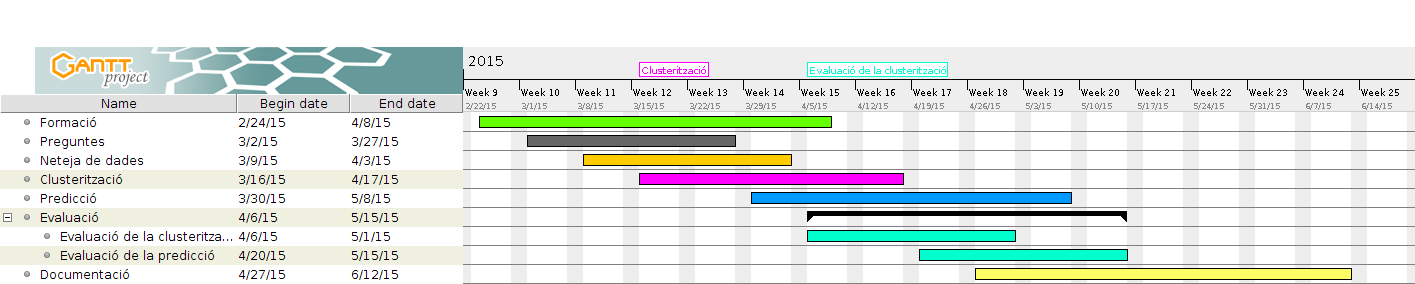
\includegraphics[width=\linewidth]{img/initialplanification.png}
\caption{Planificació inicial}
\label{fig:planificacioinicial}
\end{center}
\end{figure}


\begin{figure}[h]
\begin{center}
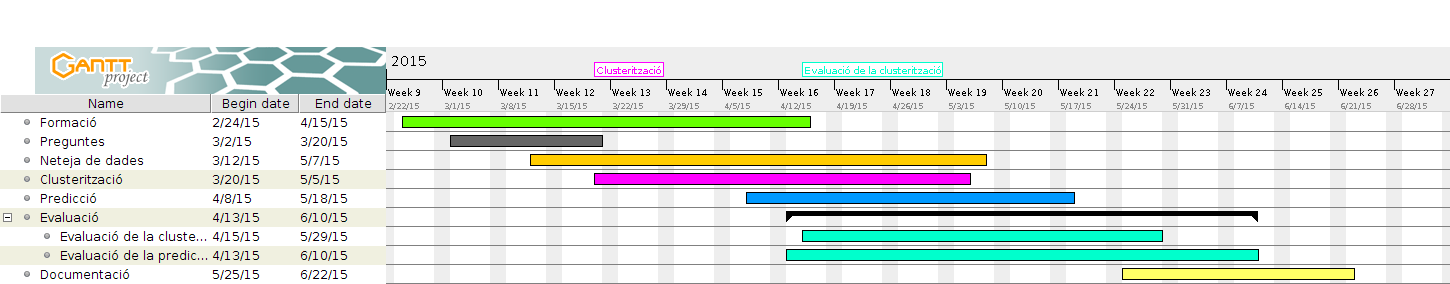
\includegraphics[width=\linewidth]{img/realplanification.png}
\caption{Planificació real}
\label{fig:planificacioreal}
\end{center}
\end{figure}

S'observa que s'ha pogut seguir la planificació inicial, tot i que en el cas de la neteja de dades s'ha allargat el temps. Això és degut a l'espera de noves revisions de dades.
\\
\\
El Treball de Fi de Grau equival a 18 crèdits ECTS. Si cada crèdit equival a 25 hores, llavors tenim:

$$18\,cr\grave{e}dits \cdot \frac{25\,hores}{1\,cr\grave{e}dits} = 450\,hores$$

\newpage

Per tant totes les tasques s'han de realitzar en 450 hores. Les hores dedicades han sigut les següents:

\begin{table}[h]
\centering

\begin{tabular}{@{}llllllll@{}}
      & \rotatebox{90}{Formació} & \rotatebox{90}{Preguntes} & \rotatebox{90}{Neteja de dades} & \rotatebox{90}{Clusterització} & \rotatebox{90}{Predicció} & \rotatebox{90}{Avaluació} & \rotatebox{90}{Documentació} \\ \midrule
Hores & 25       & 25        & 50              & 75             & 75        & 125       & 50           \\ \bottomrule
\end{tabular}
\caption{Hores de dedicació per cada tasca}
\end{table}

\subsection{Avaluació económica}

\begin{table}[h]
\centering

\begin{tabular}{@{}llll@{}}
\toprule
                & Hores & Preu per hora (Euro) & Preu total (Euro) \\ \midrule
Formació        & 25    & 0                 & 0              \\
Plantejament de preguntes       & 25    & 10                & 250            \\
Neteja de dades & 50    & 20                & 1000           \\
Clusterització  & 75    & 25                & 1875           \\
Predicció       & 75    & 25                & 1875           \\
Avaluació       & 125   & 25                & 3125           \\
Documentació    & 75    & 0                 & 0              \\ \midrule
TOTAL           & 450   &                   & 8125           \\ \bottomrule
\end{tabular}
\caption{Taula d'avaluació económica}
\end{table}

El projecte sortiria per 8125 euros, en els quals s'inclou en la etapa d'avaluació, una documentació dels resultats obtinguts i les conclusions d'aquests.

\newpage

\section{Desenvolupament del projecte}
\subsection{Eines}
\subsubsection{Eines de suport}
Aquestes són les eines de suport que ens han ajudat al llarg del treball per tal de fer més còmode la seva organització tant personal com per equip.

\paragraph{GitHub}
GitHub \cite{github} és una plataforma online per desenvolupar projectes software de forma col·laborativa. Aquesta plataforma utilitza un control de versions anomenat Git. La finalitat de GitHub és l'emmagatzenament massiu de projectes amb codi font obert. Per això hem optat per la utilització de GitHub, ja que volem que el nostre codi el pugui veure tothom i que qualsevol que el necessiti per fer la seva investigació, el pugui utilitzar.

\paragraph{Bitbucket}
Bitbucket \cite{bitbucket} és una plataforma semblant a GitHub, però amb el servei d'un altre control de versions com Mercurial a més de Git. Bitbucket té l'advantatge de permetre crear repositoris privats de forma gratuïta. Aquesta plataforma va bé per a l'inici d'un projecte on es fan molts canvis en el codi, ja que es pot tenir el codi en privat, i un cop el codi està més madur, es pot migrar a GitHub. Això és el que hem fet nosaltres en el projecte, començar amb Bitbucket i després passar-ho a GitHub amb el codi font obert.

\paragraph{Trello}
Per últim, com eina de suport hem fet servir Trello \cite{trello}, una plataforma online que permet una comunicació més clara entre els membres d'un projecte. Amb Trello es poden crear projectes i cada projecte conté un conjunt de llistes que s'omplen amb tasques. Hem fet servir Trello per tenir present una planificació i per organitzar-nos millor.

\newpage
\subsubsection{Eines de programació}
En aquesta secció ens trobarem amb el llenguatge de programació, i conjunt de biblioteques informàtiques, que hem treballat.

\paragraph{Python}
Python \cite{python} és un llenguatge d'alt nivell interpretat. Remarquen molt la fàcil lectura del seus codis, per això té una sintaxis molt semblant a un pseudocodi. Python és un llenguatge de codi obert i desenvolupat per \textit{Python Software Foundation}, una organització sense ànim de lucre. Vam escollir Python per dues raons: per ser un llenguatge de scripting i per les seves biblioteques informàtiques relacionades amb el tractament de dades (com \hyperlink{pandas}{Pandas}, \hyperlink{numpy}{NumPy} o \hyperlink{sklearn}{Scikit-learn}).


\hypertarget{pandas}{
	\paragraph{Pandas}
}
Pandas \cite{pandas} és una biblioteca informàtica escrita en Python per a la manipulació i anàlisi de dades. Especialment va bé per al tractament de taules alhora de fer consultes, o per a l'agrupació i agregació d'informació.

\hypertarget{numpy}{
	\paragraph{NumPy}
}
Numpy \cite{numpy} és una biblioteca informàtica de Python per operar amb vectors i matrius d'una forma més extensa de la que et permet el llenguatge Python. Numpy conté tot un conjunt de funcions matemàtiques d'alt nivell per treballar amb aquests vectors i matrius.

\hypertarget{sklearn}{
	\paragraph{Scikit-learn}
}
Scikit-learn \cite{sklearn} (o sklearn) és una biblioteca informàtica orientada a l'aprenentatge automàtic per a Python. Té suport per classificadors, regressors i clusterització. Per aquest projecte hem fet servir clustering i regressors. En la secció de \hyperlink{tecniquesutilitzades}{Tècniques utilitzades} es detalla cada tècnica que s'utilitza d'aquesta biblioteca informàtica.

\newpage

\paragraph{Bokeh}
Bokeh \cite{bokeh} és una biblioteca informàtica per a la visualització interactiva de dades dirigida als navegadors per a la seva presentació a través d'HTML i JavaScript. Bokeh té el suport per a gràfiques específiques com diagrames de barra, \textit{box} plots o \textit{time series}, però a banda d'aquests gràfics podem dibuixar sobre un gràfic amb elements bàsics com cercles, línies o rectangles, entre d'altres.

\paragraph{Seaborn}
Per últim tenim Seaborn \cite{seaborn} que també és una biblioteca informàtica per a visualitazció de dades com Bokeh, amb gràfiques específiques per a la visualització de resultats estadístics. A més té una part dedicada a les paletes de colors, la qual permet escollir un conjunt de colors afavorits per mostrar les dades.


\subsubsection{Eines d'edició}
\paragraph{IPython notebook}
Ipython notebook \cite{ipythonnotebook} és un editor per a l'entorn de Python. La filosofia \textit{notebook} s'empra per tenir un codi molt més llegible i a més tenir explicacions d'allò que es programa, ja que es pot barrejar codi, la sortida del codi, markdown i HTML. Hem optat per escollir aquest entorn d'edició ja que en un projecte de ciència de les dades s'ha de veure resutats constants i poder-los comentar.

\paragraph{Texmaker}
Texmaker \cite{texmaker} és una eina d'edició de \LaTeX, la qual permet poder generar informes, documents i llibres d'una forma més programàtica. A partir d'un etiquetatge estipulat es poden generar documents amb un estil predefinit com el d'aquesta memòria.

\newpage
\hypertarget{tecniquesutilitzades}{
	\subsection{Tècniques utilitzades}
}

A continuació es presenten les tècniques i mètriques de clusterització i predicció de dades utilitzades en aquest projecte. La finalitat és proporcionar un coneixement per poder passar a la secció d'\textit{Experiments i resultats} [secció:~\ref{sec:experimentsiresultats}].

\subsubsection{Tècniques de clusterització}
La clusterització (o agrupacions) és molt important en el món de les dades, permet reconèixer diferents grups de ítems de les nostres dades, en el nostre cas d'alumnes. Per això, abans de veure els resultats i experiments explorats, cal entendre les diferències entre les diferents tècniques de clusterització. En aquest projecte hem fet servir dues tècniques, on l'objectiu d'elles és el mateix, fer agrupacions de les dades i trobar diferents grups d'alumnes. Aquestes dues tècniquies són K-means i MeanShift, ambdues implementades en la biblioteca informàtica de Scikit-learn.

\paragraph{\textit{K-means}}
\textit{K-means} \cite{k-means} probablement és un dels algoritmes d'agrupació més conegut. Partint de $n$ elements, divideix aquests $n$ elements en $k$ grups (argument obligatòri de l'algoritme) on cada element pertany al grup més proper a la mitjana. L'algoritme de \textit{K-means} està descrit de la següent forma:
\\
\\
Tenint un conjunt d'elements $\mathbf{(x_1, x_2, \ldots, x_n)}$ on cada elements és un vector $d$ dimensional, \textit{K-means} construeix una partició dels elements en $k$ grups, on $k \leq n$ quedant $\mathbf{S} = \{S_1, S_2, \ldots, S_k\}$. Amb la finalitat de minimitzar la suma dels quadrats dins de cada grup:

$$ \underset{\mathbf{S}} {arg\,min} \sum_{i=1}^{k} \sum_{\mathbf{x} \in S_i} \left\| \mathbf{x} - \mu_i \right\|^2 $$

on $\mu_i$ és el centroide dels punts del conjunt $S_i$, és a dir, el punt mig.
\\
\\
Com es veu en la fórmula, aquest algoritme depén d'una $k$, per determinar agrupacions, per tant \textit{K-means} ha de rebre com paràmetre d'entrada quants grups busquem. També podem pensar que depén del centroide $\mu_i$, però no es necessari, ja que aquest convergeix si s'itera sobre la fórmula.

\newpage

\paragraph{\textit{Mean Shift}}
\textit{Mean Shift} \cite{mean-shift} és l'altre tècnica d'agrupació o clusterització que s'utilitza en aquest projecte. L'objectiu d'aquesta tècnica és el mateix que \textit{K-means}, però el seu algoritme funciona de forma diferent, considerant l'espai de característiques com una funció de densitat de probabilitat.
\\
\\
Aquest algoritme no necessita com a entrada el número de clusters que busquem, com \textit{K-means}. En la Figura \ref{fig:meanshiftvskmeans} podem veure la diferència entre \textit{K-means} i \textit{Mean Shift}.

\begin{figure}[h]
\centering
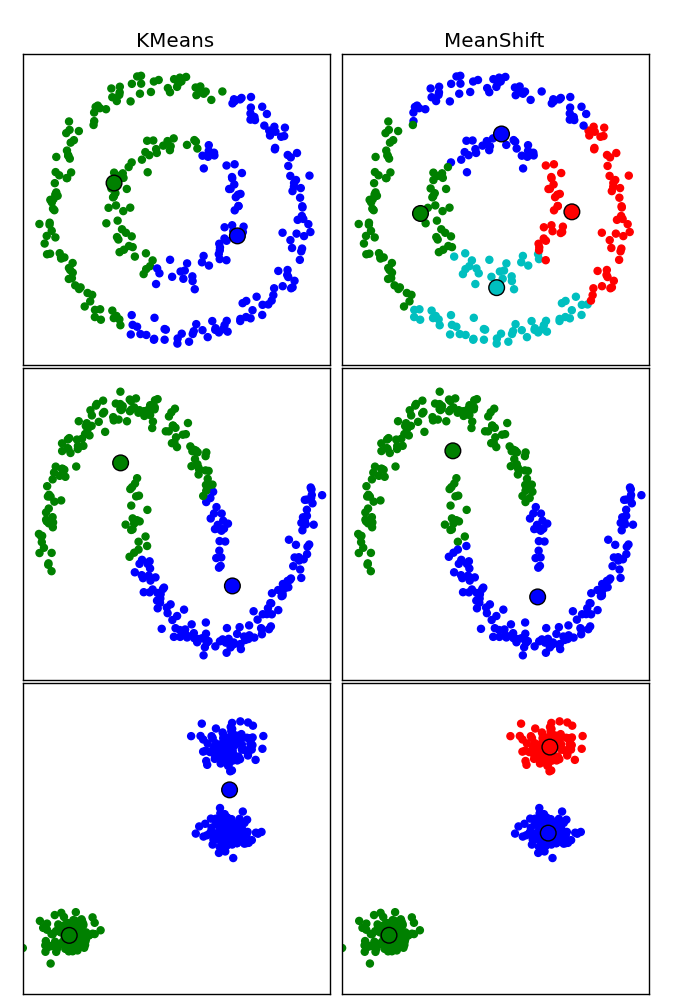
\includegraphics[width=.4\linewidth]{img/kmeansVsMeanshift.png}
\caption{Comparació de K-means amb Mean Shift \cite{comp-meanshift-kmeans}}
\label{fig:meanshiftvskmeans}
\end{figure}

Com es veu en la Figura \ref{fig:meanshiftvskmeans}, tercera fila, en no ser necessari especificar el número d'agrupacions que volem a \textit{MeanShift}, ell mateix ens diu que hi ha tres grups. Però en canvi, amb \textit{K-means} si l'apliquem amb $k=2$, per exemple, estaríem unificant dos clusters reals en un.

\newpage

\paragraph{Mètriques per al clustering}
Existeixen dos indicadors d'avaluació dels resultats de l'anàlisi:
\begin{enumerate}
	\item \textbf{Supervisat} Utilitza les agrupacions reals per comparar-les amb les agrupacions donades per l'algoritme de clusterització.
	\item \textbf{No supervisat} Mesura la qualitat del propi model, basant-se en les característiques d'aquest.
\end{enumerate}

En el nostre cas, el que volem és explorar i averiguar quins perfils d'estudiants hi ha, per tant hem d'utilitzar mètriques no supervisades, ja que no tenim una referència per comparar. La mètrica no supervisada utilitzada és la \textit{Silhouette}.

\subparagraph{\textit{Mètrica de Silhouette}}
Silhouette \cite{silhouette} és una mesura no supervisada, que valora la integritat de cada cluster dins d'un cluster. Per cada punt (o observació) calculem la \textit{silhouette} amb la següent fórmula:

$$ s(i) = \frac{b(i) - a(i)}{\max\{a(i),b(i)\}} $$

on:
\begin{itemize}[leftmargin=.5in]
	\item [$i$] és el punt del qual volem calcular la \textit{silhouette}.
	\item [$a(i)$] és la distància mitja als altres punts dins del cluster de $i$.
	\item [$b(i)$] és la distància mitja als punts que no estan dins del cluster de $i$.
\end{itemize}

Un cop tenim la \textit{silhouette} calculada per cada observació, per tenir la \textit{silhouette} de tots els clusters, fem la mitja de totes elles.

$$ \mathrm{silhouette} = \frac{1}{n} \sum_{j=1}^n s(i) $$

\newpage


\subsubsection{Tècniques de predicció}
\label{subsec:predictors}
L'etapa de predicció és important en un projecte de ciència de les dades, ja que ens permet predir el futur d'una forma estadística en base a les observacions que tenim. Però igual que la clusterització, hi ha diverses tècniques. Aquí explicaré quines tècniques hem utilitzat per aquest treball.
\\
\\
Un predictor és un algoritme que passat un conjunt de dades d'entrenament, és capaç de poder predir dades del futur. En el nostre cas, entrenem als predictors amb les notes de primer i segon de carrera. Llavors si li passem un alumne amb les notes de primer, el predictor ens podrà predir quines seran les seves notes de segon basant-se en les dades que li hem passat prèviament per entrenar.

\paragraph{Recomanador}
Unes de les tècniques per predir dades són els recomanadors. En aquest apartat s'explica com funciona el recomanador que hem definit per al context del nostre projecte. Tenint en compte les notes d'un conjunt d'alumnes, el recomanador será capaç de predir de forma estadística les notes d'un alumne en base a la resta.
\\
\\
Donada una matriu de notes de la següent forma:
$$
C = \bordermatrix{~ &         a_1   &    a_2   &   \cdots    &    a_m  \cr
                  e_1    &  c_{11}  &     ?    &   \cdots    &  c_{1m} \cr
                  e_2    &  c_{21}  &  c_{22}  &   \cdots    &    ?    \cr
                  \vdots &  \vdots  &  \vdots  &   \ddots    &  \vdots \cr
                  e_n    &    ?     &  c_{n2}  &   \cdots    &  c_{nm} \cr
                  }
$$

on:
\begin{itemize}[leftmargin=.5in]
	\item [$e_i$] és un estudiant.
	\item [$a_i$] és una assignatura.
	\item [$c_{ij}$] és la nota de l'estudiant $i$ en l'assignatura $j$.
	\item [$?$] són notes no completes, perquè un alumne no ha cursat l'assignatura.
\end{itemize}

La finalitat del recomanador, és omplir la matriu de notes allà on aparegui '$?$' i col·locar la nota més adient. Abans d'explicar com funciona, s'introduirà els diferents tipus de recomanadors que hi ha.

\subparagraph{1 - Recomanador col·laboratiu basat en l'estudiant (RCxE)}
Prediem la nota d'un alumne en base a la semblança amb la resta. És a dir, si un alumne $e_i$ té unes notes semblants a un alumne $e_j$, les assignatures que no ha cursat $e_i$, es pot dir que seran semblants a les notes que ha tret $e_j$ en aquelles assignatures.

\subparagraph{2 - Recomanador col·laboratiu basat en assignatures (RCxA)}
En comptes de basar-nos en la semblança entre els estudiants, ens basem en la semblança entre una assignatura amb la resta. És a dir, si una assignatura $a_i$ segueix una distribució semblant a una assignatura $a_j$, llavors podem dir que un alumne $e_i$ treurà una nota semblant en ambdues assignatures.

\subparagraph{3 - Recomanador híbrid}
Per últim tenim la barreja dels dos recomanadors esmentats, aplicant un pes d'importància a cadascun. Aquest recomanador no s'ha fet servir en aquest projecte, però es podria fer servir si es pogués apendre quin pes assignar a cada tipus de recomanador.
\\
\\
Ara s'eplicarà el recomanador col·laboratiu basat en l'estudiant, el qual agafem com a base per explicar el basat en assignatures. Imaginem que tenim una matriu semblant a la d'abans:
\\
$$
C = \bordermatrix{~      &   a_1   & \cdots  &           a_q            & \cdots  &   a_m  \cr
                  e_1    &  c_{11} & \cdots  & \textbf{c}_{\textbf{1q}} & \cdots  &    ?   \cr
                  \vdots &  \vdots & \ddots  &     \textbf{\vdots}      & \iddots & \vdots \cr
                  e_p    &    ?    & \cdots  &       \textbf{?}         & \cdots  & c_{pm} \cr
                  \vdots &  \vdots & \iddots &       \textbf{\vdots}    & \ddots  & \vdots \cr
                  e_n    &  c_{n1} & \cdots  & \textbf{c}_{\textbf{nq}} & \cdots  & c_{nm} \cr
                  }
$$
\\

Volem predir la nota que conté el símbol $?$ en negreta a la posició $c_{pq}$. S'ha d'aplicar la següent fórmula a la posició que es vol predir la nota:
$$
	c_{pq} = \sum_{i=1}^n{\alpha(e_i, e_p) c_{iq}}
$$
on:
\begin{itemize}[leftmargin=.5in]
	\item [$e_i$] és un estudiant.
	\item [$a_i$] és una assignatura.
	\item [$\alpha$] és una funció de similitud normalitzada, que dóna pes a $c_{iq}$.
\end{itemize}

Amb aquesta fórmula podem veure la funcionalitat d'aquest recomanador, si ens fixem, com més semblants siguin dos estudiants, més pes li donarem a la nota que ha tret un dels dos per recomanar-li a l'altre. Això és la fórmula d'una mitja ponderada.
\\
\\
Si el que volem és fer un recomanador basat en assignatures, tenim dues opcions. O bé aplicar la següent fórmula:
$$
	c_{pq} = \sum_{j=1}^n{\alpha(a_j, a_q)c_{pj}}
$$
O bé, fer la transposada de la matriu anterior i aplicar la mateixa fórmula d'abans.
\\
\\
Per construïr aquest recomanador col·laboratiu s'ha de modelar seguint l'interfaç dels predictors de la biblioteca informàtica de \textit{Scikit-learn}. Un predictor en \textit{sklearn} ha de tenir un mètode \textit{fit} i un altre que sigui \textit{predict}. En la Figura \ref{fig:codiexemple} es pot veure el fluxe de les crides a les funcions.

\begin{figure}[h]
\begin{minted}
[
framesep=5mm,
baselinestretch=1.2,
bgcolor=bgcode,
fontsize=\footnotesize
]
{python}
from sklearn.linear_model import LinearRegression
# Definim les variables
X = [(1,2,3), (5,3,2), (3,1,0), (123,433,452), (233,231,786)]
# Fem el promig per cada Xi
y = [2, 3.33, 1.33, 336, 416]
# Definim una nova variable
x = (45,34,65) # promig = 48
# Creem un predictor
predictor = LinearRegression()
predictor.fit(X,y)
print predictor.predict(x)
# >> 47.9271056831
\end{minted}
\caption{Fluxe de crides de funcions d'un predictor d'sklearn}
\label{fig:codiexemple}
\end{figure}

\newpage

Primer s'ha de cridar al mètode \textit{fit} i seguidament ja podem cridar al mètode \textit{predict} tantes vegades com volguem predir.

\begin{figure}[h]
\begin{minted}
[
framesep=5mm,
baselinestretch=1.2,
bgcolor=bgcode,
fontsize=\footnotesize
]
{python}
class Recomender(BaseEstimator):
    def __init__(self, method=coefPearson, transpose=False):
        self._m = None
        self._method = method
        self._transpose = transpose
        
    def fit(self, X, y):
        # ...
        return self
    
    def predict(self, X):
        # ...
        return predicted
\end{minted}
\caption{Estructura del recomanador col·laboratiu}
\label{fig:recomenderstructure}
\end{figure}

En la Figura \ref{fig:recomenderstructure} podem veure l'estructura del recomanador col·laboratiu que s'ha construït seguint la fórmula explicada anteriorment. El constructor accepta per paràmetre la funció de similitud entre items (per defecte el coeficient de pearson), i un boleà que determina si és un Recomanador col·laboratiu basat en l'estudiant (\textit{transpose=False}) o un Recomanador col·laboratiu basat en assignatures (\textit{transpose=True}).

\newpage

\paragraph{\textit{Random Forest Regressor} (RFR)}
Abans d'explicar la tècnica de \textit{Random Forest Regressor}, s'ha d'entendre el concepte d'un arbre de regressió. Un arbre de regressió és una tècnica utilitzada en aprenentatge automàtic, que es defineix com un model predictiu que mapeja observacions sobre una característica a conclusions sobre el valor objectiu d'aquesta característica. En aquestes estructures d'arbre, les fulles representen un valor real d'aquella característica i les branques les conjuccions de caracterítiques que han portat fins a la fulla.
\\
\\
\begin{figure}[h]
\centering
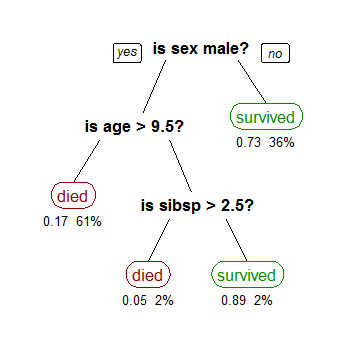
\includegraphics[width=.5\linewidth]{img/randomforest.png}
\caption{Exemple d'arbre de regressió \cite{imgrandomforestregressor}}
\end{figure}

\textit{Random Forest Regressor} \cite{randomforestregressor} és un conjunt d'arbres de regressió, on el seu resultat és la mitja de la sortida de cada arbre. A més, per a cada arbre s'aplica un soroll aleatori a les dades sense variar la seva mitja i variància. Això permet que aplicant el promig de la sortida de cada arbre de regressió, aquesta tècnica obtingui beneficis.

\newpage

\paragraph{Regressor lineal (LR)}
Un regressor lineal \cite{linearregressor} modelitza una recta de regressió a partir d'un núvol de punts. La recta definida, és la recta més propera que passa per tots els punts. El que busca és definir una variable dependent a partir d'un conjunt de variables independents, és a dir:
$$
y =\beta_0+\beta_1 x_1+\beta_2 x_2+ \cdots + \beta_n x_n + \varepsilon
$$

on $\beta_i$ són termes constants i $n$ són els conjunts d'observacions que tenim. En el cas d'una sola variable depenent, tindríem un resultat semblant al de la Figura \ref{fig:linearregressor}.

\begin{figure}[h]
\centering
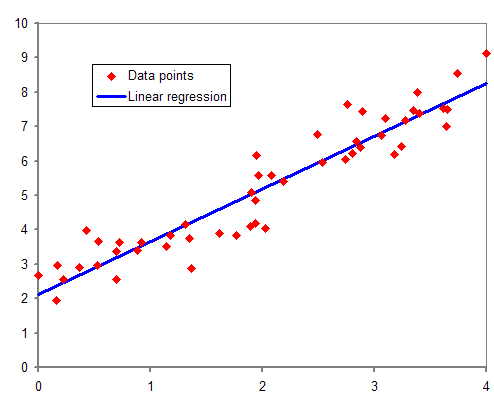
\includegraphics[width=.5\linewidth]{img/linearregression.png}
\caption{Regressió lineal \cite{imglinearregressor}}
\label{fig:linearregressor}
\end{figure}

\paragraph{Mètriques per a la predicció}
\label{par:metriquespredictors}
Igual que en la secció de clusterització, per a la predicció de dades, també hem utilitzat mesures per validar les nostres prediccions. Aquí hem utilitzat mesures supervisades. Anomenem $y_{pred}$ al conjunt de qualificacions que s'ha predit d'un alumne, i $y_{test}$ al conjunt de qualificacions real de l'estudiant.

\subparagraph{Error promig absolut (MAE)}
L'error promig absolut \cite{mae} és una mesura supervisada que es basa en fer la mitja dels errors produïts pel predictor. Està definit per la següent fórmula:
$$ \mathrm{MAE} = \frac{1}{n}\sum_{i=1}^n \left| y_{pred_i}-y_{test_i}\right| $$

\subparagraph{Error promig quadràtic (MSE)}
L'error promig quadràtic \cite{mse} és una mesusa supervisada també. Aquesta mètrica penalitza els error alts, ja que la diferència s'eleva al quadrat. La fórmula és la següent:

$$\mathrm{MSE}=\frac{1}{n}\sum_{i=1}^n(y_{pred_i}-y_{test_i})^2$$

\subparagraph{Coeficient de Pearson (PCC)}
El coeficient de Pearson, l'utilitzem com una mètrica supervisada i la fem servir per mesurar la diferència de la distribució de les notes predites amb les notes reals. El coeficient de Pearson està definit per la següent fórmula:
$$\mathrm{PCC} =\left| \frac{\sum_{i=1}^n(y_{pred_i} - \bar{y}_{pred_i})(y_{test_i} - \bar{y}_{test_i})}{\sqrt{\sum_{i=1}^n(y_{pred_i} - \bar{y}_{pred_i})^2  \sum_{i=1}^n(y_{test_i} - \bar{y}_{test_i})^2}}\right|$$

\subparagraph{Desviació estàndard (std)}
També calculem la desviació estàndard per veure si els errors són més o menys dispersos. La fórmula utilitzada és la següent:

$$ \sigma = \sqrt{ \frac{1}{n} \sum_{i=1}^n (\left| y_{pred_i}-y_{test_i}\right| - \mu)^2 } $$
\\
\\
Totes aquestes mètriques són necessàries per avaluar cada tècnica de predicció que utilitzem. Tot i així, les tècniques més importants i que tenen més pes són l'error promig absolut i el quadràtic.

\subsubsection{Tècnica de rànquing}
Un dels objectius d'aquest treball és desenvolupar un rànquing d'assignatres per a l'alumne ordenades per la seva dificultat. 
\\
\\
Per construïr el rànquing necessitem prèviament definir un predictor que ens predigui les notes d'un alumne tenint en compte un històric de qualificacions. Un cop tenim les notes que estima el predictor d'un alumne, s'ordenen aquestes de major a menor, és a dir, de menor a major dificultat. D'aquesta manera ens queda una taula d'assignatures ordenada per dificultat a la que anomenem rànquing.

\paragraph{Mètriques per al rànquing}
A continuació veurem la mètrica utilitzada per a l'avaluació de rànquings.

\subparagraph{\textit{Mean Ranking Score (MRS)}}
\label{subpar:mrs}
Està basada en la mesura d'\textit{Error promig absolut}, però amb valors discrets. És una mesura supervisada per tal de mesurar com de bo és un rànquing que s'hagi predit. Es tracta d'una mitja a partir de les distàncies d'error en el rànquing. La métrica presenta la següent fórmula:

$$ \mathrm{MRS} = \frac{1}{n}\sum_{i=1}^n \left| p(y_{pred_i}) -  p(y_{test_i})\right| $$

on:
\begin{itemize}[leftmargin=.5in]
	\item [$p$] és una funció que ens retorna la posició de l'element en el rànquing
\end{itemize}

La millor manera d'entendre aquesta mètrica és mostrar un exemple a partir d'aquesta taula:

\begin{table}[h]
\centering
\begin{tabular}{@{}cc@{}}
\toprule
Rànquing Real & Rànquing Predit \\ \midrule
A1           & A4             \\
A2           & A2             \\
A3           & A1             \\
A4           & A3             \\ \bottomrule
\end{tabular}
\caption{Exemple de rànquings}
\end{table}

Per aquest exemple, hauríem de recòrrer els 4 elements i calcular les distàncies entre les posicions reals i predites:
	$$\left|p(A1_{notes_r}) - p(A1_{notes_p})\right| = \left| 1 - 3 \right| = 2$$
	$$\left|p(A2_{notes_r}) - p(A2_{notes_P})\right| = \left| 2 - 2 \right| = 0$$
	$$\left|p(A3_{notes_r}) - p(A3_{notes_p})\right| = \left| 3 - 4 \right| = 1$$
	$$\left|p(A4_{notes_r}) - p(A4_{notes_pr})\right| = \left| 4 - 1 \right| = 3$$

Quedant:

$$ \mathrm{MRS} = \frac{2 + 0 + 1 + 3}{4} = \frac{6}{4} = 1.5$$

Ens podem fixar que si comparem dos rànquings iguals, llavors $\mathrm{MRS}$ serà igual a $0$. Per tant, com més proper estigui a 0, millor s'aproparà la predicció del rànquing real.

\subsubsection{Tècniques de reducció de dimensions}
Una de les últimes tècniques que utilitzem en aquest Treball de Fi de Grau és la reducció de dimensions. Aquest tipus de tècnica són útils per poder visualitzar dades que tinguin una dimensió major que 3. A més, aquestes tècniques permeten reduïr el cost computacional dels algoritmes basats en les dades, i en molts casos sense variar significativament en el seu resultat. Una de les tècniques utilitzades en aquest projecte és l'anàlisi de components principals (PCA).

\paragraph{PCA}
L'anàlisi de components principals o PCA \cite{pca}, el que fa és escollir un nou sistema de coordenades a partir d'una transformació lineal on s'ordenen les variàncies per mida. La variància amb major mida s'escollirà com eix principal, la segona variància com a segon eix, així successivament fins obtenir la dimensionalitat escollida.

%http://web.media.mit.edu/~tristan/phd/dissertation/chapter5.html

\newpage

\section{Experiments i resultats}
\label{sec:experimentsiresultats}
En aquest apartat s'explicarà pas per pas els experiments realitzats i els resultats obtinguts per cada pregunta plantejada a la secció [secció:\ref{subsec:preguntesplantejades}]. Fins ara s'han presentat tots els conceptes necessaris per poder entendre aquesta secció. Primer es mostren les preguntes relacionades amb la clusterització i es finalitza amb els resultats obtinguts de la predicció de notes.

\subsection{Preparació prèvia als experiments}
Abans de començar a comentar els resultats, s'explicaran quines són les dades per respondre cada pregunta. Inicialment tenim tota una taula on cada fila és la qualificació d'un alumne donada un assignatura, per tant en cada fila tenim informació com \textit{l'identificador d'alumne, assignatura, tipus d'apunt (convalidada, ordinaria o de reconeixement), qualificació de l'assignatura,} \ldots A partir d'aquesta taula fem una conversió de tal manera que en cada fila ens queda un alumne i cada columna una assignatura, construint una matriu així:

$$
\mathrm{C} = \bordermatrix{ &         a_1   &    a_2   &   \cdots    &    a_m  \cr
                  e_1    &  c_{11}  &  c_{12}  &   \cdots    &  c_{1m} \cr
                  e_2    &  c_{21}  &  c_{22}  &   \cdots    &  c_{2m}    \cr
                  \vdots &  \vdots  &  \vdots  &   \ddots    &  \vdots \cr
                  e_n    &  c_{n1}  &  c_{n2}  &   \cdots    &  c_{nm} \cr
                  }
$$
on:
\begin{itemize}[leftmargin=.5in]
	\item [$e_i$] és un estudiant.
	\item [$a_j$] és una assignatura.
	\item [$c_{ij}$] és la nota de l'alumne $i$ donada una assignatura $j$.
\end{itemize}

$C\in \mathbb{R}^{n \times n}$ on $0 \leq c_{ij} \leq 10$, la matriu no conté cap nombre desconegut i cada alumne $e_i$ ha cursat tot el conjunt d'assignatures $\{a_1, a_2, a_3, \ldots, a_m\}$.
\\
\\
El conjunt d'assignatures que apareixen en les columnes pot variar depenent de la pregunta que volem respondre, pot ser el conjunt d'assignatures de primer, com el conjunt de les de primer més les de segon. Però a partir d'una matriu com aquesta ens basarem en algunes qüestions.

\newpage
\subsection{Perfils d'estudiants}
\label{subsec:perfilsestudiants}
La resposta a la pregunta: \textit{Hi ha diferents perfils d'alumnes?} és trobar diferents tipus d'estudiants en relació a la seva nota. Alumnes amb notes molt bones en tot, alumnes amb notes dolentes en certes assignatures i alumnes que suspenen, entre d'altres. Però volem que el nostre algoritme explori els grups que poden haver-hi de forma no supervisada, és a dir, sense indicar-li quins són els grups a priori.
\\
\\
Com que el que busquem són grups d'alumnes amb qualificacions semblants, utilitzarem la tècnica de \textit{K-means}. Aquesta tècnica és capaç d'agrupar alumnes en relació a la distància de les seves notes. \textit{K-means} té una limitació, necessita com argument el número de clusters $(k)$ que volem trobar. Hem de buscar una forma de poder trobar la millor $k$.
\\
\\
La primera opció és aplicar \textit{K-means} amb diferents \textit{k} i per cada prova, calcular la mesura de \textit{Silhouette}. Es calcula la \textit{silhouette} perquè volem saber com de disgregat està cada perfil i determinar si els perfils són robustos. L'algoritme de \textit{K-means} rep com a paràmetre una matriu com la matriu $C$ amb els alumnes que hagin cursat totes les assignatures de primer de cada grau implantat en la Facultat de Matemàtiques de la Universitat de Barcelona. 

\begin{figure}[h]
\centering
\begin{subfigure}{.45\textwidth}
  \centering
  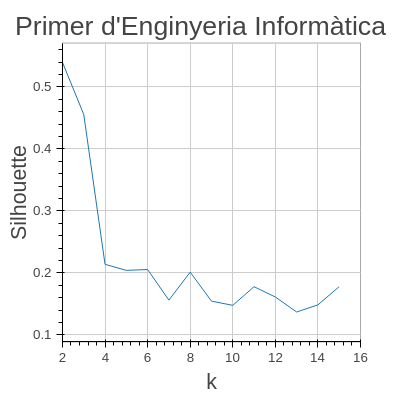
\includegraphics[width=\linewidth]{img/silhouette_primer_info.png}
  \caption{Enginyeria Informàtica}
\end{subfigure}
\begin{subfigure}{.45\textwidth}
  \centering
  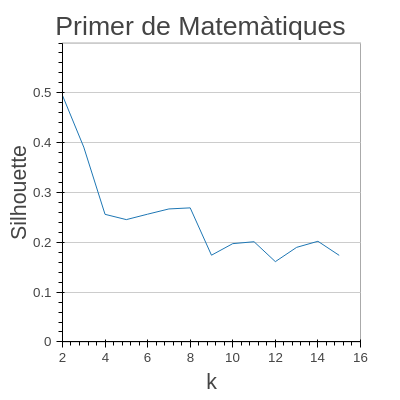
\includegraphics[width=\linewidth]{img/silhouette_primer_mates.png}
  \caption{Matemàtiques}
\end{subfigure}
\caption{Càlcul de la mesura \textit{Silhouette}}
\label{fig:silhouettekmeans}
\end{figure}

Els gràfics de la Figura \ref{fig:silhouettekmeans} ens diuen que la millor $k$ en ambdós casos és $k=2$ i la mesura de silhouette descendeix conforme augmenta el paràmetre $k$. Tanmateix, aquest resultat amb $k=2$ no és interessant per al nostre anàlisi perquè busquem un número de clusters major que 2, encara que els clusters siguin menys disgregats. Podem opinar que la mesura \textit{silhouette} és major amb $k=2$ perquè les notes es separen molt bé en aprobats i suspesos, sobretot al primer curs de cada grau. Però nosaltres volem explorar més perfils, per tant hem de buscar una altre forma per determinar quina és la millor $k$.
\\
\\
L'altre solució proposada és reduïr la dimensionalitat de les dades per tal de poder visualitzar-les en un pla dos-dimensional. D'aquesta manera podrem veure visualment els grups que tenim per cada curs. Apliquem la tècnica de PCA per reduïr de 10 dimensions a 2. Com a suport visual, apliquem un algoritme de clusterització, així com \textit{Mean Shift}, per tal de diferenciar millor els perfils. 

\begin{figure}[h]
\centering
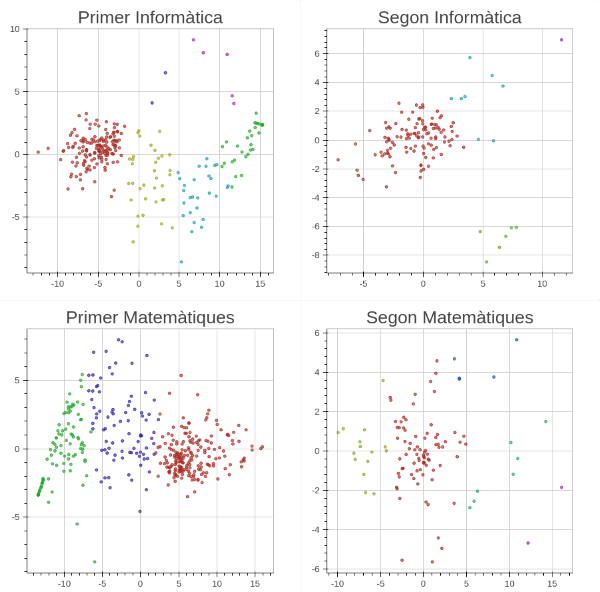
\includegraphics[width=.9\linewidth]{img/pca_info_mates.png}
\caption{Visualització dels alumnes en un espai dos-dimensional}
\label{fig:pca-meanshift}
\end{figure}

\newpage

Com es pot veure a la Figura \ref{fig:pca-meanshift}, tenim diferents perfils per cada gràfica. Passem a discutir quina és la millor $k$ per cada curs.

\subparagraph{Primer d'Enginyeria Informàtica}
Es pot separar tot el conjunt de punts en 6 agrupacions (\textit{vermell, beix, blau claret, verd, lila i blau fosc}), però els grups \textit{blau fosc} i \textit{lila} són dos grups tan reduïts i separats de la resta que els podríem comptar com un de sol cluster: $k=5$

\subparagraph{Segon d'Enginyeria Informàtica}
Per a aquest curs separem als estudiants en 4 grups, i podem veure que els clusters estan força disgregats entre ells i no fa falta unificar cap:  $k=4$

\subparagraph{Primer de Matemàtiques} 
Per a primer del grau de Matemàtiques separem les observacions en 3 clusters. Com no es veu cap anomalia, a part de la petita separació dels petits punts verds, podem considerar els tres clusters:  $k=3$

\subparagraph{Segon de Matemàtiques}
Aquest és el curs amb el que hem tingut més problemes, perquè els punts estan més distanciats entre ells i això fa que no es pugui interpretar el número de clusters per aplicar \textit{K-means}. En l'anàlisi de perfils veurem que el número de clusters òptim és 3: $k=3$
\\
\\
Ara que ja tenim el valor de $k$ adequat per cada curs, podem aplicar la tècnica de \textit{K-means}. S'ha utilitzat una combinació de colors adequada per cada perfil, veure Figura \ref{fig:colorsperfils}.

\begin{figure}[h]
\centering
\begin{subfigure}{.2\textwidth}
  \centering
  
\includegraphics[width=\linewidth]{img/aprovats.png}
  \caption{Aprovats}
\end{subfigure}
\begin{subfigure}{.2\textwidth}
  \centering
  
\includegraphics[width=\linewidth]{img/bonesnotes.png}
  \caption{Bones notes}
\end{subfigure}
\begin{subfigure}{.2\textwidth}
  \centering
  
\includegraphics[width=\linewidth]{img/suspesos.png}
  \caption{Suspesos}
\end{subfigure}
\begin{subfigure}{.2\textwidth}
  \centering
  
\includegraphics[width=\linewidth]{img/altresperfils.png}
  \caption{Altres}
\end{subfigure}
\caption{Categoria de colors utilitzada per representar els perfils d'estudiants}
\label{fig:colorsperfils}
\end{figure}

\newpage

Comentem els resultats obtinguts amb el curs de primer d'Enginyeria Informàtica on hem aplicat \textit{K-means} amb $k=5$.

\begin{figure}[h]
\centering
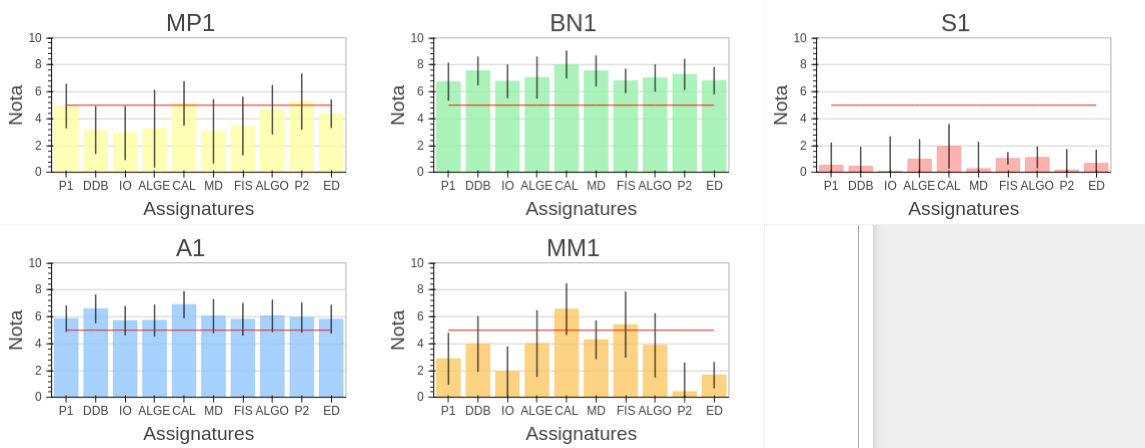
\includegraphics[width=\linewidth]{img/perfils_primer_info.png}
\caption{Perfils d'alumnes de primer d'Enginyeria Informàtica}
\label{fig:perfilsprimerinfo}
\end{figure}

\begin{figure}[h]
\centering
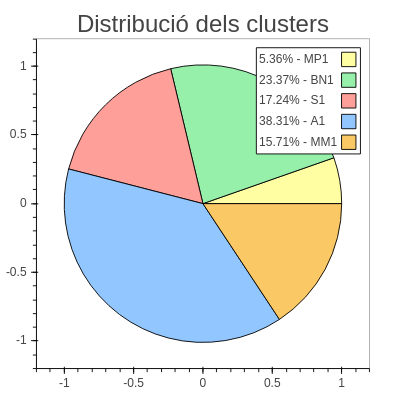
\includegraphics[width=.55\linewidth]{img/perfils_primer_info_pastilla.png}
\caption{Percentatges de cada agrupació}
\label{fig:pasprimerinfo}
\end{figure}

Cada gràfic de la Figura \ref{fig:perfilsprimerinfo} correspon als diferents perfils d'estudiants que ha trobat la tècnica de \textit{K-means}. En cadascun d'ells trobem com a títol l'etiqueta assignada a aquell perfil, i el color de cadascún depén de la seva categoria (Figura \ref{fig:colorsperfils}). En l'eix d'abscisses es veuen les assignatures (en aquest cas les de primer d'Enginyeria Informàtica), i en l'eix d'ordenades la mitja de les notes dels alumnes de cada assignatura (longitud de la barra). Per últim les línies negres determinen la desviació estàndard de la distribució de cada assignatura i la línia vermella és una marca per identificar l'alçada de l'aprovat. En la Figura \ref{fig:pasprimerinfo} es mostra el percentatge d'alumnes que pertanyen a cada agrupació.
\\
\\
Els perfils explorats del primer curs d'Enginyeria Informàtica es descriuen de la següent manera:



\subparagraph{1 - BN1: Bones notes de primer d'Informàtica}
Aquest perfil correspon als alumnes que tenen bones notes en totes les assignatures de primer i com podem veure en el gràfic de pastilla, representen un 23.37\% del total, sent el segon perfil més abundant. Donat que la mostra és més gran, la desviació estàndard és menor, és a dir, aquest perfil és força estable. Tots els estudiants que hi pertanyen es distancien amb una qualificació promig d'1.5 aproximadament.

\subparagraph{2 - S1: Suspesos de primer d'Informàtica}
Com podem veure, aquest perfil són els estudiants que suspenen la majoria d'assignatures. A priori podem pensar que són els que solen deixar la carrera i és això el que anem a respondre en la següent pregunta plantejada. També podem veure que són un 17.24\% del total d'alumnes que han cursat les assignatures de primer.

\subparagraph{3 - A1: Aprovats de primer d'Informàtica}
Són la major part dels alumnes, amb un 38.31\% del total, i són els alumnes que de mitja treuen entre 5 i 7 en totes les assignatures. Igual que passa amb el cluster \textit{BN1}, la desviació estàndard de cada assignatura és força baixa, i això fa que el cluster sigui consistent.

\subparagraph{4 - MP1: Millors en programació de primer d'Informàtica} 
Aquest perfil encaixa amb els alumnes que tenen millors notes en les assignatures de programació que en les de matemàtiques. La distribució d'aquests és molt dispersa, això ho podem veure per la llargada de la barra negra (desviació estàndard). La mostra és petita, representa el 5.36\% de la mostra total.

\subparagraph{5 - MM1: Millors en Matemàtiques de primer d'Informàtica}
Aquest perfil igual que \textit{MP1}, és bastant inestable, ja que tenen una desviació estàndard alta, és a dir, hi ha una diversitat elavada de notes. Tot i que siguin dispersos, són un 15.71 \% del total, un percentatge forç alt.
\\
\\
Si mirem el resultats en general de les gràfiques de la Figura \ref{fig:perfilsprimerinfo}, podem veure que l'assignatura \textit{Estructura de Dades} (ED) presenta sempre una desviació més petita que la resta d'assignatures en cada perfil, és a dir, que les notes es concentren més en la mitja marcada. També es veu en tots els perfils, sense mirar la qualificació corresponent, que la nota més alta correspon a l'assignatura de \textit{Càlcul} (CAL).
\\
\\
Seguint amb l'anàlisi, a la Figura \ref{fig:perfilssegoninfo} podem veure els perfils de tots els alumnes que han cursat totes les assignatures de segon. S'ha aplicat \textit{K-means} amb $k=4$.

\begin{figure}[h]
\centering
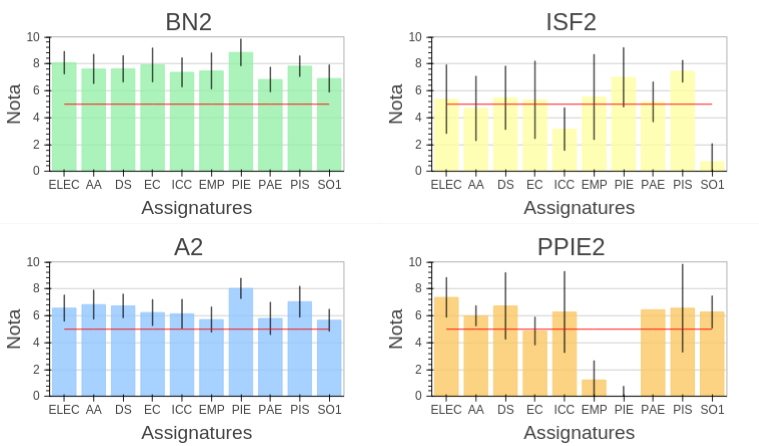
\includegraphics[width=.8\linewidth]{img/perfils_segon_info.png}
\caption{Perfils d'alumnes de segon d'Enginyeria Informàtica}
\label{fig:perfilssegoninfo}
\end{figure}

\begin{figure}[h]
\centering
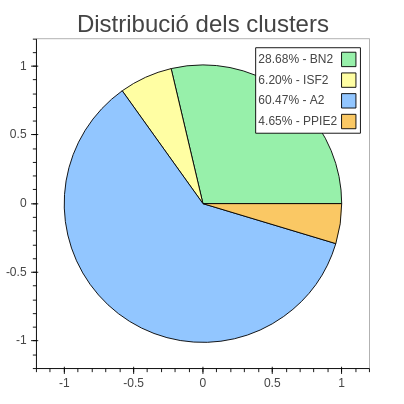
\includegraphics[width=.4\linewidth]{img/perfils_segon_info_pastilla.png}
\caption{Percentatges de cada agrupació}
\end{figure}


Els perfils explorats del segon curs d'Enginyeria Informàtica es descriuen de la següent manera:

\subparagraph{1 - BN2: Bones notes de segon d'Informàtica}
Aquest és un perfil força semblant a \textit{BN1}, és per això que ens plantejem, a la secció \ref{subsec:conservacioclusters}, la pregunta: \textit{Amb quin perfil de provinença encaixa cadascun d'aquests perfils?} És cert que els que tenen bones notes a primer, solen ser els que treuen bones notes a segon? Això ho anomenem conservació de clusters. De tots els alumnes que han cursat segon un 28.68\% pertanyen a aquest cluster, més d'un quart de la mostra.

\subparagraph{2 - A2: Aprovats de segon d'Informàtica}
Aquest perfil és semblant al perfil \textit{A1}, pertany als alumnes que tenen notes entre 5 i 7 en totes les assignatures. Són el 60.47\% del total d'alumnes que han cursat les assignatures de segon d'Enginyeria Informàtica.

\subparagraph{3 - ISF2: ICC i SO1 fluixes}
Aquest perfil encara que sigui minoritari, amb un 6.2\% del total, és força curiós, ja que són alumnes que tenen \textit{Introducció a la Computació Científica} (ICC) i \textit{Sistemes operatius I} (SO1) amb notes més baixes que la resta. S'ha de dir que tot i que les mitjes siguin més petites, les desviacions estàndard són molt altes, el que fa que les notes dels alumnes siguin més diverses i no segueixin exactament la distribució de mitjes del perfil.

\subparagraph{4 - PPIE2: Problemes amb PIE i Empresa}
Aquest és el perfil amb un percentatge més petit de població, un 4.65\%. És un perfil força dispers, ja que les desviacions estàndard són altes, i això es pot veure en assignatures com PIS o ICC. A més és curiós perquè és un grup que apareix amb les assignatures d'\textit{Empresa} (EMP) i \textit{Probabilitat i estadística} (PIE) suspeses.
\\
\\
Ens podem fixar que la distribució de mitjes del perfil \textit{BN2} i \textit{A2}, és força semblant, només que \textit{BN2} té les mitjes més altes.
\\
\\
Deixant enrere al grau d'Enginyeria Informàtica, passem a analitzar els estudiants del grau en Matemàtiques. Comencem amb els alumnes de primer, els quals els segmentem en 3 agrupacions ($k=3$).

\newpage

En la Figura \ref{fig:perfilsprimermates} i \ref{fig:pasprimermates}, presentem els perfils i els percentatges de les agrupacions, respectivament.

\begin{figure}[h]
\centering
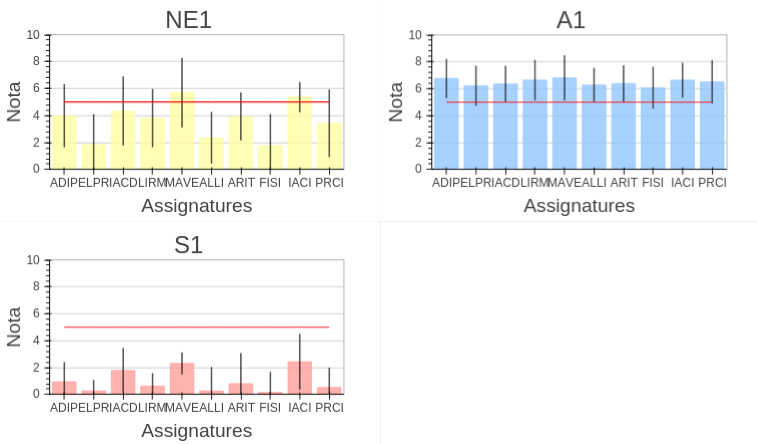
\includegraphics[width=.9\linewidth]{img/perfils_primer_mates.png}
\caption{Perfils d'alumnes de primer de Matemàtiques}
\label{fig:perfilsprimermates}
\end{figure}

\begin{figure}[h]
\centering
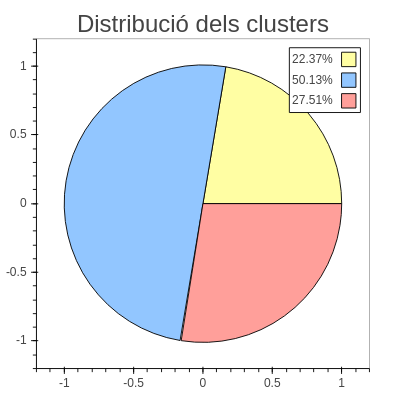
\includegraphics[width=.4\linewidth]{img/perfils_primer_mates_pastilla.png}
\caption{Percentatges de cada agrupació}
\label{fig:pasprimermates}
\end{figure}

\newpage

Els perfils explorats de primer curs de Matemàtiques es descriuen de la següent manera:

\subparagraph{1 - A1: Aprovats de primer de Matemàtiques}
Aquest perfil pertany als estudiants que tenen totes les assignatures aprovades  de mitja i són els que formen la major part del total, amb un 50.13\%.

\subparagraph{2 - S1: Suspesos de primer de Matemàtiques}
Per últim tenim els alumnes que de mitja suspenen totes les assignatures. Conformen un 27.51\% del total d'estudiants.

\subparagraph{3 - NE1: No estables de primer de Matemàtiques}
Podem veure que aquest cluster té les mostres molt distanciades, per les desviacions estàndard que presenta. Aquest perfil l'hem classificat com \textit{No estables de primer}, ja que són alumnes que amb prou feines poden aprovar certes assignatures. Conformen un 22.37\% del total d'estudiants.
\\
\\
Per últim s'observa els alumnes de segon de Matemàtiques a la Figura \ref{fig:perfilssegonmates} i \ref{fig:passegonmates}.

\begin{figure}[h]
\centering
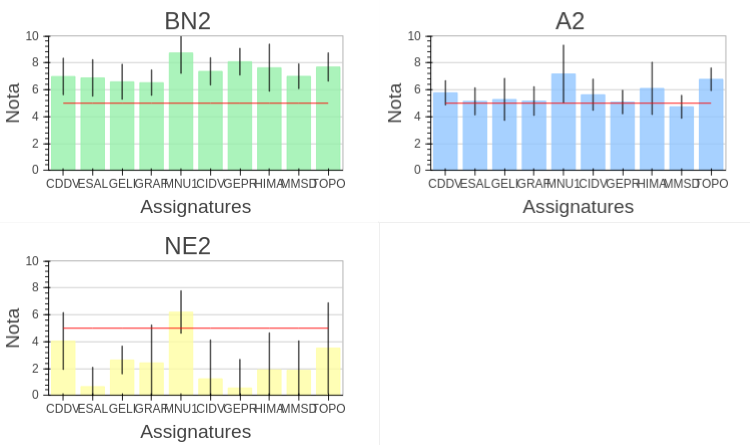
\includegraphics[width=.85\linewidth]{img/perfils_segon_mates.png}
\caption{Perfils d'alumnes de segon de Matemàtiques}
\label{fig:perfilssegonmates}
\end{figure}

\begin{figure}[h]
\centering
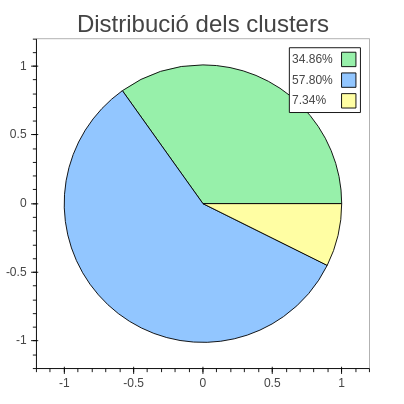
\includegraphics[width=.4\linewidth]{img/perfils_segon_mates_pastilla.png}
\caption{Percentatges de cada agrupació}
\label{fig:passegonmates}
\end{figure}

\newpage

Els perfils explorats de segon curs de Matemàtiques es descriuen de la següent manera:

\subparagraph{1 - BN2: Bones notes de segon de Matemàtiques}
Torna a aparèixer aquest tipus de perfils corresponent a alumnes amb mitjes de qualificacions altes. Tot i així, el percentatge d'alumnes que pertanyen a aquest cluster és elevat, un 34.86\%. Aquest fet fa pensar que totes les assignatures suposen la mateixa dificultat per aquests alumnes.

\subparagraph{2 - A2: Aprovats de segon de Matemàtiques}
Novament tenim als alumnes amb qualificacions en el rang d'aprovat, tot i que la majoria freguen la línea de l'aprovat. Com és en tots els cursos, aquest és el perfil més abundant, amb un 57.80\%.

\subparagraph{3 - NE2: No estables de segon de Matemàtiques}
Igual que a primer del grau de Matemàtiques tenim el perfil de \textit{No estables}. Aquí el tornem a tenir, tot i que aquest perfil només té aprovada per mitja una assignatura, \textit{Mètodes numèrics I} (MNU1). Pertanyen al 7.34\% del total.
\\
\\
En aquest curs tenim un efecte semblant a primer d'Enginyeria Informàtica amb l'assignatura de \textit{Càlcul}, hi ha una assignatura que en tots els perfils correspon a la mitja més alta, \textit{Mètodes numèrics I} (MNU1).
\\
\\
Arran d'aquests resultats, el tutor d'estudis pot aplicar l'acció de reforçar l'aprenentatge i el seguiment de tots aquells alumnes que s'agrupen en perfils on la majoria d'assignatures no passin de la línia vermella de l'aprovat.

\newpage

\subsection{Taxa d'abandonament per perfil}
La primera pregunta que ens plantegem és: \textit{Quina és la taxa d'abandonament per cada tipus de perfil?} És cert que els que suspenen abandonen la carrera? Ara ho podrem demostrar amb gràfics estadístics. Ens centrarem en la taxa d'abandonament dels alumnes que cursen primer, tant d'Enginyeria Informàtica com el grau de Matemàtiques. Mostrarem els perfils, Figura \ref{fig:tap}, per poder discutir cada perfil amb la seva taxa d'abandonament, mostrada a la Figura \ref{fig:abandonamentprimer}.

\begin{figure}[h]
\centering
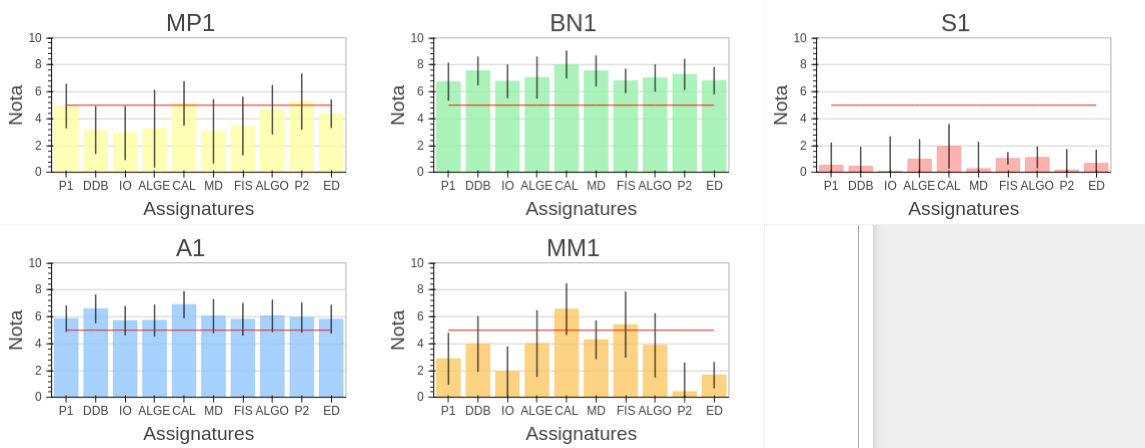
\includegraphics[width=\linewidth]{img/perfils_primer_info.png}
\caption{Perfils d'alumnes de primer d'Enginyeria Informàtica}
\label{fig:tap}
\end{figure}

\begin{figure}[h]
\centering
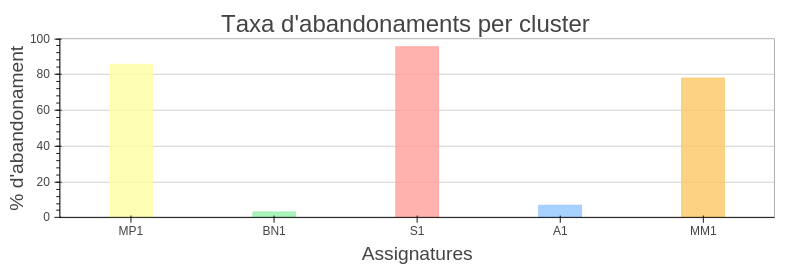
\includegraphics[width=\linewidth]{img/abandonaments_primer_info.png}
\caption{Taxa d'abandonaments per perfil de primer d'Enginyeria Informàtica}
\label{fig:abandonamentprimer}
\end{figure}

Els alumnes que amb més probabilitat deixen la carrera són els que suspenen (S1), seguits d'estudiants que no tenen unes notes massa estables (MP1 i MM1). És a dir, que la majoria que passen a segon pertanyen al cluster \textit{BN1} i \textit{A1}. Però si ens fixem en el gràfic d'abandonaments, els perfils d'aprovats (A1) i de bones notes (BN1), hi ha un petit percentatge indicat que diu que abandonen la carrera. En les dades que tenim, no tenim un camp que ens indiqui si un alumne ha abandonat la carrera o no, ja que no ho tenen registrat. Hem hagut d'agafar per cada perfil tot el conjunt d'alumnes d'aquell perfil i s'ha comprovat per cadascun si té assignatures matriculades a l'any següent. Però clar, hi ha alumnes del darrer any que s'han de matricular per l'any vinent encara (i no apareixen matriculats a l'any següent), per això hi ha un petit marge d'error i els clusters \textit{BN1} i \textit{A1} aparèixen amb una mínima taxa d'abandonaments degut a aquest error.
\\
\\
Per altra banda, tenim el curs de primer de Matemàtiques, on apliquem el mateix algoritme explicat en el paràgraf anterior. També trobem un petit marge d'error en els perfils que ho aproven tot.

\begin{figure}[h]
\centering
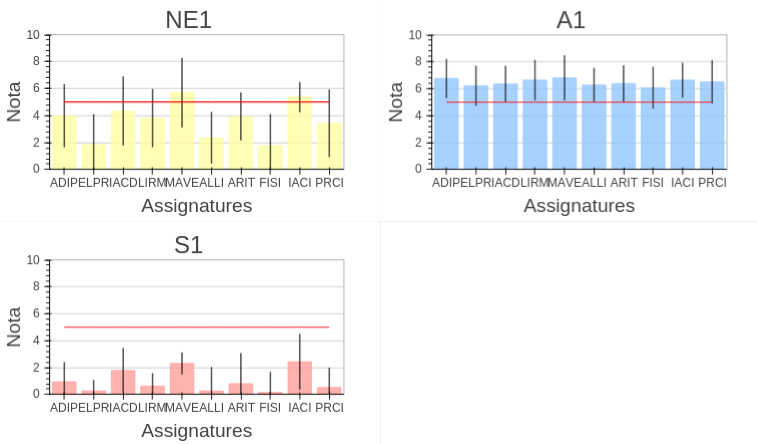
\includegraphics[width=0.9\linewidth]{img/perfils_primer_mates.png}
\caption{Perfils d'alumnes de primer de Matemàtiques}
\end{figure}

\begin{figure}[h]
\centering
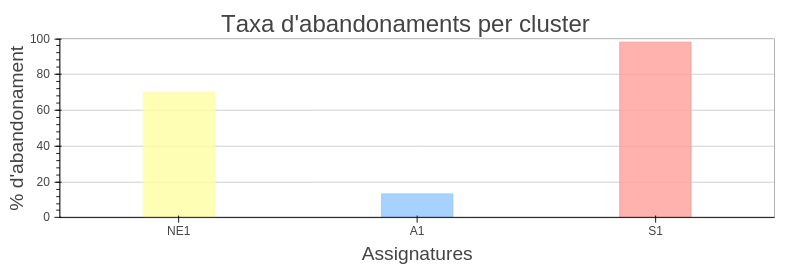
\includegraphics[width=.9\linewidth]{img/abandonaments_primer_mates.png}
\caption{Taxa d'abandonaments per perfil de primer de Matemàtiques}
\label{fig:tappm}
\end{figure}

A la Figura \ref{fig:tappm} presentem la taxa d'abandonament dels alumnes de primer del grau de Matemàtiques. Igual que en Enginyeria Informàtica, ens trobem que la major taxa d'abandonament es troba en els alumnes que suspenen per mitja totes les assignatures (S1). Seguidament els hi segueixen els estudiants que no tenen unes notes massa regulars i com s'ha comentat anteriorment, els alumnes que estan classificats com \textit{Aprovats}, també surten amb una taxa mínima d'abandonament.
\\
\\
Tant al grau d'Enginyeria Informàtica com al grau de Matemàtiques podríem definir una acció per al tutor. Després del primer curs, es pot incidir (enviar correus electrònics, aconsellar) als alumnes dels perfils amb baixes notes com són els grups S1, MM1 i MP1 per al grau d'Enginyeria Informàtica i S1 i NE1 per al grau de Matemàtiques.

\newpage

\subsection{Conservació de clusters}
\label{subsec:conservacioclusters}
La pregunta que ens plantegem és: \textit{Amb quin perfil de provinença encaixa cadascun d'aquests perfils?} El que es vol mirar en aquesta pregunta és la conservació de clusters, per exemple, els estudiants que treuen bones notes a primer, segueixen treien bones notes a segon? O, de quina via d'accés solen provenir els estudiants de primer de Matemàtiques? Preguntes com aquestes anem a resoldre en aquest apartat. 
\\
\\
Començarem, com hem fet anteriorment, amb els estudiants que han cursat primer d'Enginyeria Informàtica. Contrastem primer d'Enginyeria Informàtica i primer de Matemàtiques amb les vies d'accés: Batxillerat i salt d'Universitat.

\begin{figure}[h]
\centering
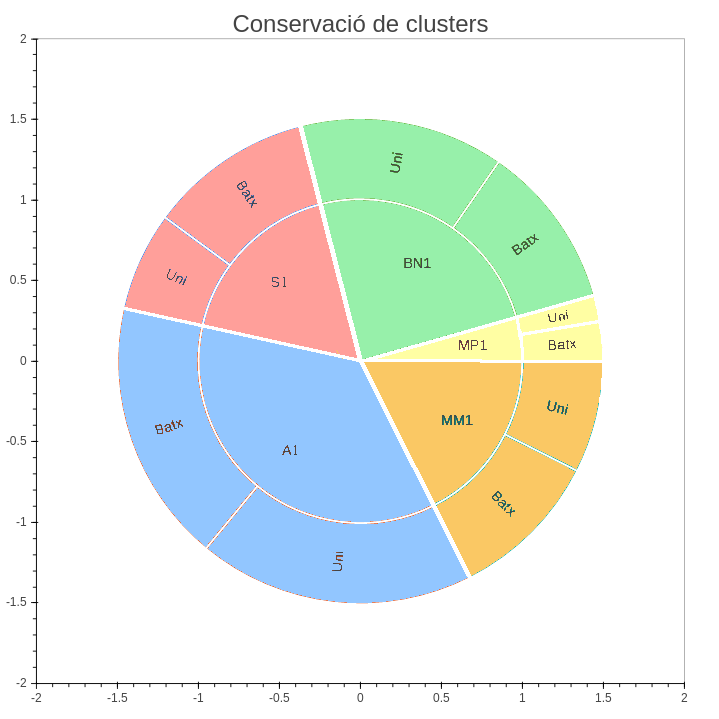
\includegraphics[width=.6\linewidth]{img/conservacio_clusters_primer_info.png}
\caption{Conservació de clusters dels alumnes de primer d'Informàtica}
\label{fig:ccei1}
\end{figure}

En la figura [\ref{fig:ccei1}] podem veure que a l'interior del cercle, tenim el mateix gràfic de pastilla que s'ha vist anteriorment dels perfils dels estudiants de primer d'Enginyeria Informàtica [fig:~\ref{fig:pasprimerinfo}]. Per fora del cercle de cada perfil es veu quantitativament d'on venen els alumnes del perfil. 
\\
\\
Es pot veure com en tots els perfils, venen meitat de Batxillerat i meitat de Salt d'Universitat aproximadament. Es pot distingir que els estudiants classificats com \textit{Suspesos} solen venir més de Batxillerat que no pas d'una altre Universitat, tot i que la diferència és petita. Com s'ha vist en la gràfica d'abandonament [fig:~\ref{fig:abandonamentprimer}], els alumnes que passen amb més abundancia a segon són els classificats com \textit{A1} i \textit{BN1}, per tant procedim a eliminar a la resta, ja que són minoria, per a que quedi més llegible en la Figura \ref{fig:ccei2}.

\begin{figure}[h]
\centering
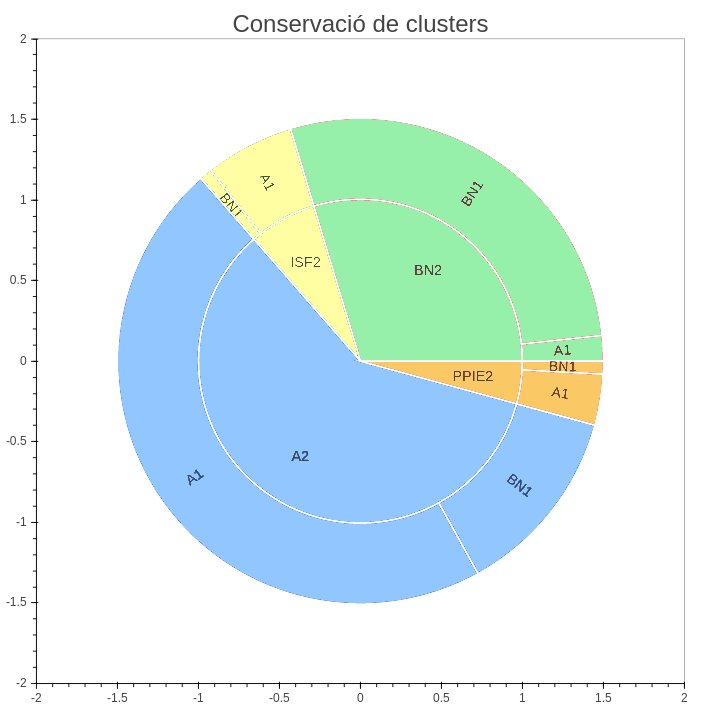
\includegraphics[width=.6\linewidth]{img/conservacio_clusters_segon_info.png}
\caption{Conservació de clusters dels alumnes de segon d'Informàtica}
\label{fig:ccei2}
\end{figure}

Ara es veu amb més claredat el significat d'un gràfic com aquest, ja que podem veure com els que solen treure bones notes a primer d'Enginyeria Informàtica, solen treure bones notes a segon també, i els que es classificaven com \textit{Aprovats de primer}, solen parar a \textit{Aprovats de segon}. També podem veure com un petit percentatge d'alumnes que treuen notes a primer, passen a treure notes més baixes a segon, igual que alumnes etiquetats com \textit{Aprovats de primer} amb una petita quanitat paren a perfils inestables com \textit{ISF2} o \textit{PPIE2}.
\\
\\
Per últim es veurà la provinença dels estudiants de primer del grau de Matemàtiques, on també es pot veure una tendència [fig:~\ref{fig:ccm1}].

\newpage

\begin{figure}[h]
\centering
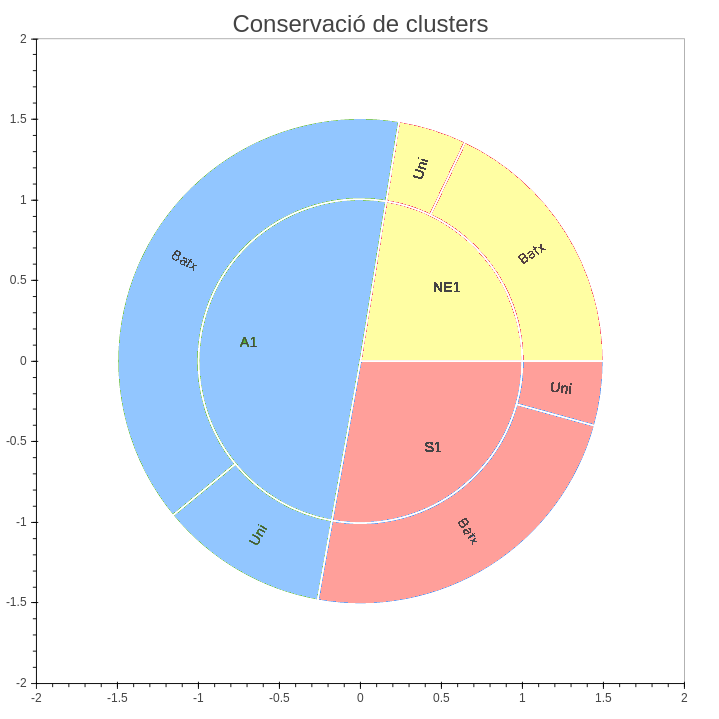
\includegraphics[width=.6\linewidth]{img/conservacio_clusters_primer_mates.png}
\caption{Conservació de clusters dels alumnes de primer de Matemàtiques}
\label{fig:ccm1}
\end{figure}

En la Figura \ref{fig:ccm1} es veu amb claredat que la major part d'estudiants que han cursat primer del grau de Matemàtiques, venen de Batxillerat. 
\\
\\
Una de les raons per les quals vam plantejar aquesta pregunta, era per saber si podiem determinar un perfil d'estudiant del grau a partir de la via d'accés d'aquest. Malauradament no s'ha trobat cap correlació com aquesta, però s'han pogut veure resultats molt coherents i que no esperavem trobar.  L'anàlisi de les dades ens ha permès extreure informació útil pels tutors d'estudis. Depenent del perfil actual de l'alumne se li podrà recomanar un material de suport a l'estudi adicional.

\newpage

\subsection{Predicció de notes i rànquing de dificultat d'assignatures}
En aquest apartat s'expliquen  les tècniques de predicció que hem fet servir i quins resultats, tant quantitatius com qualitatius, s'han obtingut. El que busquem és poder mostrar un rànquing, personalitzat per cada alumne, d'assignatures ordenades per la dificultat que li costarà a cada estudiant.
\\
\\
Abans de construïr el rànquing, necessitem saber quina és la tècnica de predicció que s'ajusta millor a les nostres dades. Les tècniques utilitzades per aquest experiment han sigut les següents, anteriorment explicades [secció:~\ref{subsec:predictors}]:

\begin{itemize}[leftmargin=.5in]
	\item Recomanador col·laboratiu basat en l'estudiant (RCxE)
	\item Recomanador col·laboratiu basat en assignatures (RCxA)
	\item \textit{Random Forest Regressor} (RFR)
	\item Regressor lineal (LR)
\end{itemize}

Anem a mesurar quantitativament quin dels 4 predictors s'adequa més a les nostres dades. Les mètriques que s'utilitzaran són les que ja s'han explicat en la secció de \textit{Mètriques de predictors} [secció:~\ref{par:metriquespredictors}].

\subsubsection{Estratègia de validació}
Totes les proves realitzades s'han fet a partir de les notes d'Enginyeria Informàtica. Per fer aquestes proves s'ha utilitzat la tècnica de \textit{cross-validation}, que  consisteix en la partició del conjunt de les dades en \textit{training} i \textit{test} de tal manera que s'entrena amb el subconjunt de \textit{training} i s'avalua amb el subconjunt de \textit{test}. Fent aquestes proves podrem comprovar quin dels predictors és el més adequat. Les proves s'han realitzat a partir de dos conjunts diferents de dades:

\begin{itemize}[leftmargin=.5in]
	\item Una on s'aplica com a \textit{training} les notes de primer d'Enginyeria Informàtica i com a \textit{test} les notes de segon. A partir d'ara l'anomenarem conjunt nº1.
	\item Per un altra banda, s'ha aplicat un \textit{training} amb les notes de primer i segon, i un \textit{test} amb les notes de tercer d'Enginyeria Informàtica. A partir d'ara l'anomenarem conjunt nº2.
\end{itemize}

Per cadascun dels conjunts s'han realitzat diferents proves, detallades a continuació:

\paragraph{Proves amb dades contínues}
Provem els predictors mirant l'error produït amb les notes reals i les predites qualificades del 0 al 10. Les mesures utilitzades en aquesta prova són:

\begin{itemize}[leftmargin=.5in]
	\item \textbf{Error Promig Absolut} Per calcular la mitja d'error produït.
	\item \textbf{Error Promig Quadràtic} Per veure si els errors són molt elevats.
	\item \textbf{Coeficient de Pearson} Per veure si la distribució entre les notes es manté.
	\item \textbf{Desviació estàndard} Utilitzada per veure si els errors es concentren o estan molt disgregats.
\end{itemize}

A més, a partir dels errors produïts per cada predictor es mostra un diagrama de caixes \cite{boxplot} per representar la distribució dels errors. Més endavant amb un dels resultats s'explica l'interpretació del diagrama de caixes. S'utilitza un 90\% de \textit{training} i un 10\% de \textit{test}.


\paragraph{Proves amb dades discretes}
Igual que comprovem l'error produït amb valors continus, del 0 al 10, ara etiquetem les notes segons el seu rang. El rang que s'ha utilitzat és el següent:

\begin{itemize}[leftmargin=.5in]
	\item \textbf{Suspés} Notes inferiors a 5 ($nota < 5$)
	\item \textbf{Aprovat} Notes entre 5 i 7 ($5 \leq nota < 7 $)
	\item \textbf{Notable} Notes entre 7 i 9 ($7 \leq nota < 9 $)
	\item \textbf{Excel·lent} Notes superiors a 9 ($nota \geq 9$)
\end{itemize}

Per poder visualitzar aquesta prova s'ha utilitzat una matriu de confusió \cite{confusionmatrix}, on es representa amb un mapa de color (o heatmap). En la següent secció s'explica que és un mapa de color juntament amb els resultats obtinguts. S'utilitza un 50\% de \textit{training} i un 50\% de \textit{test}.

\paragraph{Proves amb rànquing d'assignatures}
Per últim tenim les proves realitzades per mesurar el rànquing que volem desenvolupar. La mètrica utilitzada ha sigut la \textit{Mean Ranking Score}, que com ja s'ha explicat anteriorment [secció:~\ref{subpar:mrs}], és una mètrica que ens permet mesurar com de bó és un rànquing. S'utilitza un 90\% de \textit{training} i un 10\% de \textit{test}.

\subsubsection{Resultats de les proves amb dades contínues}
Comançarem amb les proves fetes amb dades contínues amb els dos conjunts de dades que s'ha explicat en l'apartat anterior.
\\
\begin{figure}[h]
\centering
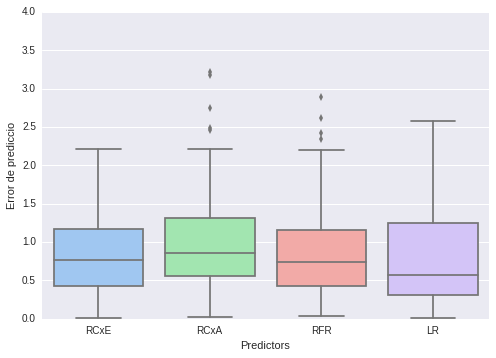
\includegraphics[width=.7\linewidth]{img/boxplot_primer_segon.png}
\caption{Prova amb dades contínues del conjunt nº1}
\label{fig:boxplotdctp}
\end{figure}

En la Figura \ref{fig:boxplotdctp} podem veure un diagrama de caixes de l'error de predicció dels diferents predictors. Aquest tipus de diagrama representa visualment una distribució. Cada caixa té les mateixes característiques: la línea del centre representa la mediana de la distribució, la caixa visualitza un 50\% de la mostra (des del primer quartil, fins el tercer), les línies verticals determinen el límit de les distribucions i, per últim, tota mostra que estigui fóra de lo normal (mostra atípica) es visualitza per fóra dels límits amb un punt.
\\
\\
La distribució que podem veure a la Figura \ref{fig:boxplotdctp} són els errors que es presenten en cada predicció. Per tant, un predictor perfecte mostrarà una distribució uniforme en el 0. En la figura es pot veure els quatre predictors utilitzats i quina distribució d'error segueix cadascun. Veiem que ele predictore més establee i que concentren millor els errors són el recomanador col·laboratiu basat en estudiant (RCxE) i el \textit{random forest regressor} (RFR). Per una altra banda, tenim el regressor lineal que presenta la mediana més baixa, tot i que el tercer quartil és massa elevat. Els \textit{outliers} (mostres atípiques) que veiem tenen una explicació. Què passa si un alumne té un imprevist i no pot cursar una assignatura ja matriculada? Aquest factor no el contemplen els predictors. És per això que tenim observacións atípiques, perquè els predictors potser prediuen que un alumne treurà un 7, però l'alumne per qualsevol raó es desmatricula de l'assignatura, llavors en aquella assignatura li queda un 0. En la Taula \ref{tab:rppcf} es mostra un exemple d'una mostra atípica amb una prova qualitativa.

Les mateixes conclusions podem extreure de les mètriques que utilitzem per fer aquesta prova:

\begin{table}[h]
\centering
\begin{tabular}{lllll}
\hline
\textit{\textbf{Algoritme$\setminus$Mètriques}} & \textbf{MAE} & \textbf{MSE} & \textbf{PCC} & \textbf{std} \\ \hline
\textbf{RCxE}          & 0.796          & 0.910          & 0.578          & 0.526          \\
\textbf{RCxA}          & 1.006          & 1.509          & 0.309          & 0.705          \\
\textbf{RFR}           & 0.868          & 1.152          & 0.505          & 0.632          \\
\textbf{LR}            & 0.809          & 1.071          & 0.575          & 0.646          \\ \hline
\end{tabular}
\caption{Mètriques per a proves quantitatives amb dades contínues del conjunt nº1}
\label{tab:mpqdctp}
\end{table}

Observem amb les mètriques que els millors predictors són RCxE, RFR i LR, tot que el presenta menys errors és RCxE ja que té l'error promig quadràtic més baix.
\\
\\
Igual que hem fet proves amb el conjunt nº1, procedim a visualitzar en la Figura \ref{fig:pdctps} i a la Taula \ref{tab:mpqdcc2} les proves amb el conjunt nº2.

\begin{figure}[h]
\centering
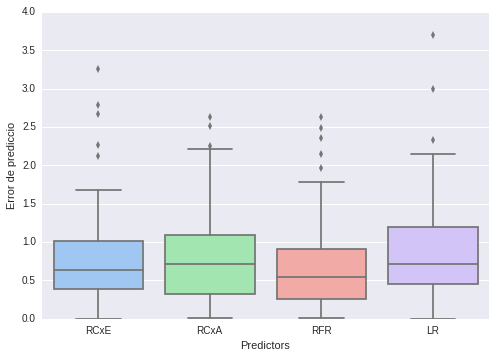
\includegraphics[width=.7\linewidth]{img/boxplot_primersegon_tercer.png}
\caption{Prova amb dades contínues del conjunt nº2}
\label{fig:pdctps}
\end{figure}

\begin{table}[h]
\centering
\begin{tabular}{lllll}
\hline
\textit{\textbf{Algoritme$\setminus$Mètriques}} & \textbf{MAE} & \textbf{MSE} & \textbf{PCC} & \textbf{std} \\ \hline
\textbf{RCxE}          & 0.869          & 1.590          & 0.276          & 0.914          \\
\textbf{RCxA}          & 0.906          & 1.781          & 0.141          & 0.980          \\
\textbf{RFR}           & 0.786          & 1.522          & 0.339          & 0.951          \\
\textbf{LR}            & 0.932          & 1.890          & 0.283          & 1.011          \\ \hline
\end{tabular}
\caption{Mètriques per a proves quantitatives amb dades contínues del conjunt nº2}
\label{tab:mpqdcc2}
\end{table}

\newpage

En la Figura \ref{fig:pdctps} s'observa com els millors predictors són el RCxE i el RFR, tot i que ara ambdós presenten més mostres atípiques. Les distribucions i els resultats són semblants als resultats provats amb les dades anteriors. L'únic predictor que marca més diferència és el Random Forest Regressor, ja que disminueix força  la mediana de la distribució, i l'error promig absolut.

\newpage

\subsubsection{Resultats de les proves amb dades discretes}

Ara passem a veure els resultats que s'han obtingut amb les notes discretes (suspés, aprovat, notable i excel·lent). Com ja s'ha explicat, la representació d'aquestes proves es fa amb una matriu de confusió, seguidament passem a descriure que representa.

\begin{figure}[h]
\centering
\begin{subfigure}{.48\textwidth}
  \centering
  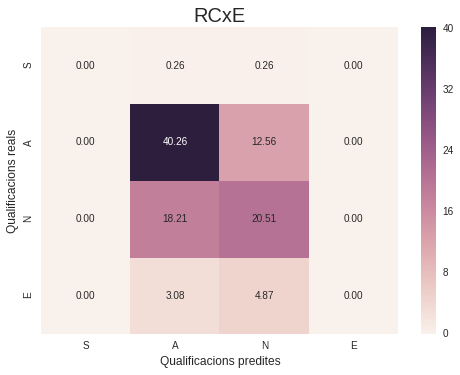
\includegraphics[width=\linewidth]{img/heatmap_rcxe_primer_segon.png}
  \caption{RCxE}
\end{subfigure}
\begin{subfigure}{.48\textwidth}
  \centering
  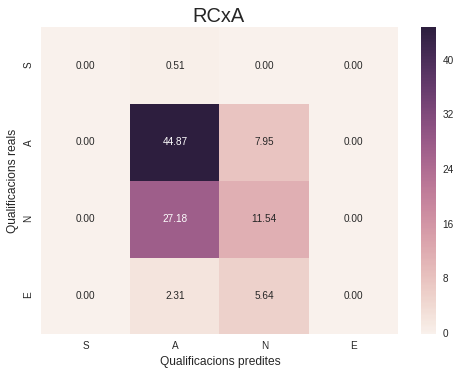
\includegraphics[width=\linewidth]{img/heatmap_rcxa_primer_segon.png}
  \caption{RCxA}
\end{subfigure}
\end{figure}
\begin{figure}[h]
\centering
\begin{subfigure}{.48\textwidth}
  \centering
  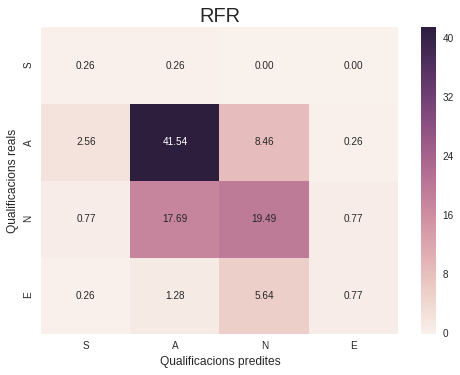
\includegraphics[width=\linewidth]{img/heatmap_rfr_primer_segon.png}
  \caption{RFR}
\end{subfigure}
\begin{subfigure}{.48\textwidth}
  \centering
  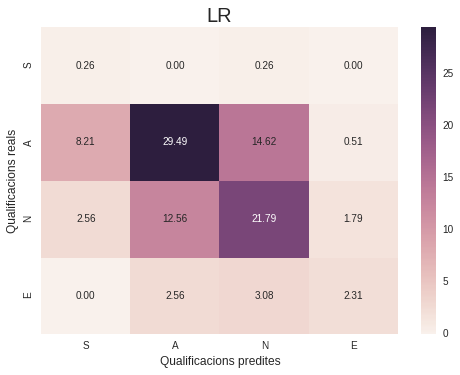
\includegraphics[width=\linewidth]{img/heatmap_lr_primer_segon.png}
  \caption{LR}
\end{subfigure}
\caption{Matriu de confusió del conjunt nº1}
\label{fig:mctp}
\end{figure}

En cada matriu de colors de la Figura \ref{fig:mctp} podem veure 16 caselles. Cada fila i columna posa: S, A, N i E, que significa: suspés, aprovat, notable i excel·lent. Cada cel·la conté el percentatge de vegades que la qualificació predita coincideix amb la qualificació real corresponent. Posem un exemple per acabar d'entendre: en la primera figura apareix en la correspondència de aprovats amb aprovats un 40.26\%, això significa que el 40.26\% de les proves realitzades, el predictor ens diu que un alumne treurà una nota d'aprovat i la nota real és aprovat. Si ens fixem, com més alt sigui el percentatge, més fosca és la casella. Per tant el que busquem és tenir fosca la diagonal, ja que vol dir que ho ha encertat tot. Ho representem amb aquest tipus de gràfic perquè equivocar-se de suspés a aprovat és acceptable, però no de suspés a excel·lent. És per això que s'ha de veure una tendencia de color a les rodalies de la diagonal.
\\
\\
Podem veure que els millors predictors són els recomanadors, ja que mantenen força alta la intensitat de color de la diagonal i el color fosc es manté concentrat a la diagonal. Si ens fixem en el \textit{Random Forest Regressor} i en el \textit{Regressor lineal} confon més per les seves rodalies. En canvi trobem que tots els predictos confonen aprovats per excel·lents.
\\
\\
Ara procedim a fer les proves amb el conjunt nº2. Els resultats són els presentats a la Figura \ref{fig:mctps}.

\begin{figure}[h]
\centering
\begin{subfigure}{.4\textwidth}
  \centering
  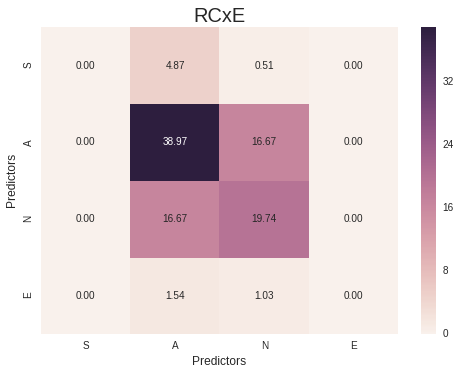
\includegraphics[width=\linewidth]{img/heatmap_rcxe_primersegon_tercer.png}
  \caption{RCxE}
\end{subfigure}
\begin{subfigure}{.4\textwidth}
  \centering
  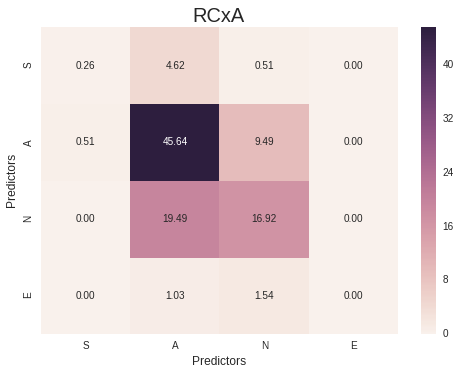
\includegraphics[width=\linewidth]{img/heatmap_rcxa_primersegon_tercer.png}
  \caption{RCxA}
\end{subfigure}
\end{figure}
\begin{figure}[h]
\centering
\begin{subfigure}{.4\textwidth}
  \centering
  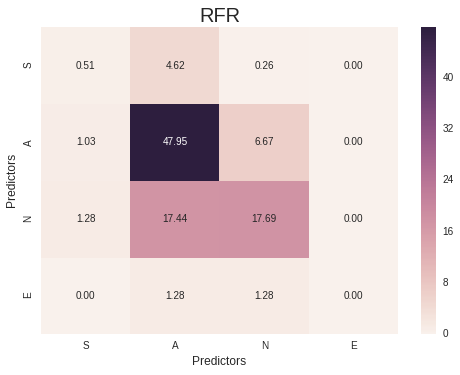
\includegraphics[width=\linewidth]{img/heatmap_rfr_primersegon_tercer.png}
  \caption{RFR}
\end{subfigure}
\begin{subfigure}{.4\textwidth}
  \centering
  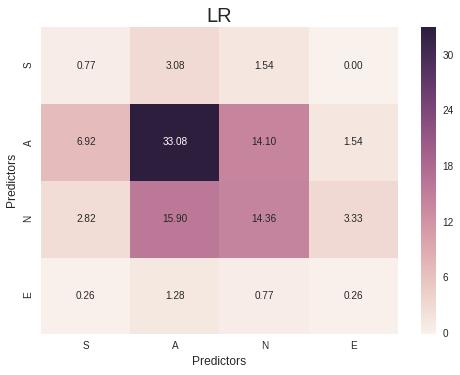
\includegraphics[width=\linewidth]{img/heatmap_lr_primersegon_tercer.png}
  \caption{LR}
\end{subfigure}
\caption{Matriu de confusió del conjunt nº2}
\label{fig:mctps}
\end{figure}

En la Figura \ref{fig:mctps} es pot veure com RCxE, RCxA i RFR tenen resultats semblants, però en canvi veiem que el regressor lineal es dispersa molt i sol fer fallades amb un salt de dos categories, com per exemple confondre notables amb suspesos. Tots ells concentren força bé els resultats a la diagonal.

\subsubsection{Resultats de les proves amb rànquing d'assignatures}
Per finalitzar la part de proves quantitatives, fem les proves pel rànquing d'assignatures. Per això s'ha utilitzat, com ja s'ha explicat, la mesura de \textit{Mean Ranking Score} per avaluar la qualitat de cada predictor i veure quin predictor és més bo per fer un rànquing. Els resultats obtinguts són purament numèrics i venen representats en la següent taula:

\begin{table}[h]
\centering
\begin{tabular}{@{}ccccc@{}}
    & \rotatebox{90}{RCxE} & \rotatebox{90}{RCxA} & \rotatebox{90}{RFR} & \rotatebox{90}{LR} \\ \midrule
MRS & 2.05                   & 2.975                   & 2.2                  & 1.975                 \\ \bottomrule
\end{tabular}
\caption{Mean Ranking Score del conjunt nº1}
\label{tab:mrstp}
\end{table}

\begin{table}[h]
\centering
\begin{tabular}{@{}ccccc@{}}
    & \rotatebox{90}{RCxE} & \rotatebox{90}{RCxA} & \rotatebox{90}{RFR} & \rotatebox{90}{LR} \\ \midrule
MRS & 2.375                   & 3.4                   & 2.375                  & 2.525                 \\ \bottomrule
\end{tabular}
\caption{Mean Ranking Score del conjunt nº2}
\label{tab:mrstps}
\end{table}

En les Taules \ref{tab:mrstp} i \ref{tab:mrstps} es poden veure els resultats de les dues proves (amb diferents \textit{training}) juntes per poder-les discutir. Recordem que la mesura MRS és una mesura que com més propera a 0, millor. Si ens fixem, els valors són més baixos a la primera taula, i el millors predictors per al conjunt nº1 són el recomanador col·laboratiu basat en l'estudiant i el regressor lineal. Amb el conjunt nº2 podem veure que els millors predictors són RCxE i RFR.
\\
\\
Podem concloure que els predictors més adequats per a les nostres dades són el RCxE i el RFR, tot i que el RCxE dóna resultats més positius. Ara procedim a fer les proves qualitatives amb el conjunt nº1 amb el RCxE, és a dir, entrenem el recomanador amb les notes de primer i avaluem amb les notes de segon.
\newpage

\subsubsection{Proves qualitatives}
En aquest apartat es mostra un cas d'èxit i un de fracàs per fer una recomanació de notes, i seguidament un cas d'èxit i un de fracàs del rànquing d'assignatures.
\\
\\
En les proves quantitatives, hem pogut veure que el millor predictor per predir notes quantitatives (de 0 a 10) és el recomanador col·laboratiu basat en l'estudiant (RCxE). És per això que utilitzarem aquest predictor per fer les proves qualitatives.

\paragraph{Resultats de les proves amb dades contínues}
Primer procedim a mostrar dos casos amb dades contínues, és a dir, agafarem les notes de primer d'Enginyeria Informàtica de dos alumnes i discutirem els resultats de la predicció amb les notes reals d'aquests.


% cas d'èxit nota quantitativa
% posar una taula com la de les hores de dedicació
% posar una taula comparant les notes predites amb les reals
\begin{table}[h]
\centering
\begin{tabular}{@{}ccccccccccc@{}}
      & \rotatebox{90}{P1} & \rotatebox{90}{DDB} & \rotatebox{90}{IO} & \rotatebox{90}{ALGE} & \rotatebox{90}{CAL} & \rotatebox{90}{MD} & \rotatebox{90}{FIS} & \rotatebox{90}{ALGO} \ & \rotatebox{90}{P2}& \rotatebox{90}{ED} \\ \midrule
Notes & 7.40 & 8.00 & 6.80 & 6.80 & 6.80 & 7.90 & 6.80 & 7.60 & 7.30 & 9.00 \\ \bottomrule
\end{tabular}
\caption{Cas d'èxit: Notes reals d'un alumne de primer}
\label{tab:nrapcedc}
\end{table}

\begin{table}[h]
\centering
\begin{tabular}{@{}lll@{}}
\toprule
     & Notes reals & Notes predites \\ \midrule
ELEC & 8.80        & 7.29           \\
AA   & 7.50        & 7.44           \\
DS   & 7.00        & 6.80           \\
EC   & 6.00        & 6.00           \\
ICC  & 6.60        & 6.74           \\
EMP  & 7.20        & 7.64           \\
PIE  & 8.00        & 6.63           \\
PAE  & 7.50        & 7.23           \\
PIS  & 9.00        & 8.81           \\
SO1  & 6.80        & 6.31           \\ \bottomrule
\end{tabular}
\caption{Cas d'èxit: Resultats de la predicció}
\label{tab:rpce}
\end{table}

\newpage

En la Taula \ref{tab:nrapcedc} es poden veure les notes reals que ha tret l'alumne en primer, i en la Taula \ref{tab:rpce} les notes que ha tret en segon juntament amb les notes predites pel predictor. Les mètriques d'aquesta predicció són:
\begin{itemize}[leftmargin=.5in]
	\item \textbf{MAE} 0.47
	\item \textbf{MSE} 0.48
\end{itemize}

Si mirem detingudament la comparació de les notes podem veure que la diferència és baixa, l'assignatura que manté una major distància és \textit{Probabilitat i Estadística} (PIE), amb una diferència d'1.37 de nota.

% cas de fracàs nota quantitativa
% posar una taula com la de les hores de dedicació
% posar una taula comparant les notes predites amb les reals
\begin{table}[h]
\centering
\begin{tabular}{@{}ccccccccccc@{}}
      & \rotatebox{90}{P1} & \rotatebox{90}{DDB} & \rotatebox{90}{IO} & \rotatebox{90}{ALGE} & \rotatebox{90}{CAL} & \rotatebox{90}{MD} & \rotatebox{90}{FIS} & \rotatebox{90}{ALGO} \ & \rotatebox{90}{P2}& \rotatebox{90}{ED} \\ \midrule
Notes & 6.00 & 8.40 & 6.00 & 6.50 & 7.10 & 7.10 & 5.50 & 7.00 & 6.00 & 6.00 \\ \bottomrule
\end{tabular}
\caption{Cas de fracàs: Notes reals d'un alumne de primer}
\label{tab:nrppcf}
\end{table}

\begin{table}[h]
\centering
\begin{tabular}{@{}lll@{}}
\toprule
     & Notes reals & Notes predites \\ \midrule
ELEC & 7.10        & 7.45           \\
AA   & 5.10        & 6.06           \\
DS   & 0.00        & 5.63           \\
EC   & 6.30        & 6.02           \\
ICC  & 5.30        & 6.38           \\
EMP  & 6.40        & 7.38           \\
PIE  & 7.30        & 6.60           \\
PAE  & 8.30        & 7.51           \\
PIS  & 0.00        & 6.89           \\
SO1  & 7.60        & 5.85           \\ \bottomrule
\end{tabular}
\caption{Cas de fracàs: Resultats de la predicció}
\label{tab:rppcf}
\end{table}

En les Taules \ref{tab:nrppcf} i \ref{tab:rppcf} podem veure un cas de fracàs, on les mètriques han donat el següent resultat:
\begin{itemize}[leftmargin=.5in]
	\item \textbf{MAE} 1.94
	\item \textbf{MSE} 8.66
\end{itemize}

Aquesta és una de les mostres atípiques que s'havien vist en els diagrames de caixa. Podem veure que realment el predictor ha encertat amb la majoria d'assignatures, llevat de PIS i DS. Resulta que l'alumne té un 0 en ambdues assignatures, això es degut a un error o per que l'alumne ha abandonat l'assignatura. El predictor no pot contemplar casos com aquest i per això presenta \textit{outliers}. En aquest cas a més podem veure com l'error promig absolut no és massa alt, però l'error promig quadràtic és elevat a conseqüència de les assignatures de \textit{Projecte integrat de Software} (PIS) i \textit{Disseny de Software} (DS).

\paragraph{Resultats de les proves amb rànquing d'assignatures}
En aquest apartat es veuen dos casos del rànquing d'assignatures, un d'èxit i l'altre de fracàs. Comencem amb el cas d'èxit presentat a les Taules \ref{tab:nrpscedc} i \ref{tab:rpscedc}.

% cas d'èxit rànquing
% posar una taula com la de les hores de dedicació
% posar una taula comparant les notes predites amb les reals
\begin{table}[h]
\centering
\begin{tabular}{@{}ccccccccccc@{}}
      & \rotatebox{90}{P1} & \rotatebox{90}{DDB} & \rotatebox{90}{IO} & \rotatebox{90}{ALGE} & \rotatebox{90}{CAL} & \rotatebox{90}{MD} & \rotatebox{90}{FIS} & \rotatebox{90}{ALGO} \ & \rotatebox{90}{P2}& \rotatebox{90}{ED} \\ \midrule
Notes & 6.00 & 6.30 & 6.00 & 6.00 & 6.50 & 6.00 & 5.50 & 6.80 & 6.00 & 6.00 \\ \bottomrule
\end{tabular}
\caption{Cas d'èxit: Notes reals d'un alumne de primer}
\label{tab:nrpscedc}
\end{table}

\begin{table}[h]
\centering
\begin{tabular}{@{}lll@{}}
\toprule
     & Notes reals & Notes predites \\ \midrule
1  & PAE         & PAE            \\
2  & PIE         & ELEC           \\
3  & EMP         & EMP            \\
4  & ELEC        & PIE            \\
5  & ICC         & AA             \\
6  & EC          & ICC            \\
7  & AA          & EC             \\
8  & SO1         & PIS            \\
9  & PIS         & SO1            \\
10 & DS          & DS             \\ \bottomrule
\end{tabular}
\caption{Cas d'èxit: Resultat de la predicció}
\label{tab:rpscedc}
\end{table}

Per determinar el millor i el pitjor cas hem hagut d'escollir els alumnes que tenien millor i pitjor mesura de \textit{Mean rànquing Score}. En la Taula \ref{tab:nrpscedc}, com els altres casos, veiem les notes que ha tret l'alumne en les assignatures de primer, però ara en la Taula \ref{tab:rpscedc} podem veure el rànquing d'assignatures ordenades per dificultat. En aquest cas s'aprecia com el rànquing predit és semblant al rànquing real. La \textit{Mean Ranking Score} dóna 1.

% cas de fracàs rànquing
% posar una taula com la de les hores de dedicació
% posar una taula comparant les notes predites amb les reals
\begin{table}[h]
\centering
\begin{tabular}{@{}ccccccccccc@{}}
      & \rotatebox{90}{P1} & \rotatebox{90}{DDB} & \rotatebox{90}{IO} & \rotatebox{90}{ALGE} & \rotatebox{90}{CAL} & \rotatebox{90}{MD} & \rotatebox{90}{FIS} & \rotatebox{90}{ALGO} \ & \rotatebox{90}{P2}& \rotatebox{90}{ED} \\ \midrule
Notes & 8.80 & 5.80 & 6.60 & 7.30 & 8.50 & 8.00 & 5.30 & 6.50 & 9.20 & 7.40 \\ \bottomrule
\end{tabular}
\caption{Cas de fracàs: Notes reals d'un alumne de primer}
\label{tab:nrpscfr}
\end{table}

\begin{table}[h]
\centering
\begin{tabular}{@{}lll@{}}
\toprule
     & Notes reals & Notes predites \\ \midrule
1    & ICC    & PIS       \\
2    & PIE    & PIE      \\
3    & PAE    & EMP       \\
4    & DS     & AA      \\
5    & ELEC   & PAE       \\
6    & SO1    & ELEC        \\
7    & EMP    & SO1       \\
8    & PIS    & EC      \\
9    & AA     & DS       \\
10   & EC     & ICC        \\ \bottomrule
\end{tabular}
\caption{Cas de fracàs: Resultat de la predicció}
\label{tab:rpscfr}
\end{table}

Per últim podem veure aquest cas de fracàs en les Taules \ref{tab:nrpscfr} i \ref{tab:rpscfr}, on els dos ranking no s'assemblen. La seva \textit{Mean Ranking Score} ens ha donat 3.8, una MRS alta i recordem que la MRS és la mitja d'error de diferència de posicions del rànquing.
\\
\\
Amb els resultats que hem arribat en aquest apartat de predicció pot ser útil per al tutor d'estudis. Pot determinar quines assignatures anirà malament un alumne i així aplicar una acció corresponent, com ara recomanar suport adicional o repàs de les matèries relacionades amb l'assignatura en qüestió.

\newpage
\section{Conclusions}
Per dur a terme aquest treball era necessari seguir les etapes d'un projecte de ciència de les dades. Hem pogut transformar les dades en coneixement, un dels objectius plantejats en aquest Treball de Fi de Grau. Fer una anàlisi estadístic sobre dades acadèmiques ens serveix com a base per al projecte d'innovació docent.
\\
\\
Com resultat de la investigació dins del marc del projecte d'innovació docent, és possible concloure resultats com l'alta conservació de perfils quan un estudiant passa de primer a segon d'Engineria Informàtica, o una alta taxa d'abandonament per part d'alumnes que suspenen les assignatures de primer. Tot i que en alguns resultats no s'ha obtingut el que s'esperava, s'han explorat nous resultats i conclusions que no s'havien arribat a tenir en compte.
\\
\\
Amb els resultats obtinguts, aquest treball pot ajudar a prendre decisions al cap d'estudis, tutors i professors dels estudis de la Facultat de Matemàtiques.

\subsection{Treball futur}
Com s'ha explicat des del principi, aquest treball entra dins del marc d'un projecte d'innovació docent, i forma part de l'anàlisi estadístic de les dades acadèmiques. El treball futur a implementar en aquest projecte són els següents punts:

\subparagraph{Desenvolupament d'un sistema intel·ligent} 
Construcció d'una eina de suport per al tutor d'estudis que li permeti explorar amb més profunditat les dades acadèmiques d'un alumne o d'una assignatura. Una de les eines a incorporar seria un sistema de visualització de les recomanacions de matrícula i gràfics estadístics que puguin ajudar a visualitzar la informació que presenten les dades.

\subparagraph{Avaluació}
Un cop construïda l'eina pel tutor, hauria de passar a fase de prova, per tal que els tutors d'estudis la provin i puguin identificar problemes o limitacions del sistema.

\newpage

\begin{thebibliography}{9}
\bibitem{pid}
``Presentació del projecte d'innovació docent" [Online]. 

Disponible: \url{http://mid.ub.edu/webpmid/content/sistema-intel\%E2\%80\%A2ligent-de-suport-al-tutor-d\%E2\%80\%99estudis}


\bibitem{normtipificada}
Normalització d'unitat tipificada - Wikipedia [Online].

Disponible: \url{https://en.wikipedia.org/wiki/Standard_score}


\bibitem{github}
Plana web de Github [Online].

Disponible: \url{https://github.com}


\bibitem{bitbucket}
Plana web de Bitbucket [Online].

Disponible: \url{https://bitbucket.org}


\bibitem{trello}
Plana web de la plataforma Trello [Online].

Disponible: \url {https://trello.com}


\bibitem{python}
Llenguatge de programació Python [Online].

Disponible: \url{https://www.python.org}


\bibitem{pandas}
Biblioteca informàtica de Python: Pandas [Online].

Disponible \url{http://pandas.pydata.org}


\bibitem{numpy}
Biblioteca informàtica de Python: Numpy [Online].

Disponible: \url{http://www.numpy.org}


\bibitem{sklearn}
Biblioteca informàtica de Python: Scikit-learn [Online].

Disponible: \url{http://scikit-learn.org}


\bibitem{bokeh}
Biblioteca informàtica de Python: Bokeh [Online].

Disponible: \url{http://bokeh.pydata.org}


\bibitem{seaborn}
Biblioteca informàtica de Python: Seaborn [Online].

Disponible: \url{http://stanford.edu/~mwaskom/software/seaborn}


\bibitem{ipythonnotebook}
Entorn de programació de Python: Ipython Notebook [Online].

Disponible: \url{http://ipython.org/notebook.html}

\bibitem{texmaker}
Editor de \LaTeX [Online].

Disponible: \url{http://www.xm1math.net/texmaker}


\bibitem{k-means}
K-means d'Scikit-learn [Online].

Disponible: \url{http://scikit-learn.org/stable/modules/generated/sklearn.cluster.KMeans.html}


\bibitem{mean-shift}
Mean Shift d'Scikit-learn [Online].

Disponible: \url{http://scikit-learn.org/stable/modules/generated/sklearn.cluster.MeanShift.html}


\bibitem{comp-meanshift-kmeans}
Imatge retocada de la plana web d'Scikit-learn [Online].

Disponible: \url{http://scikit-learn.org/stable/_images/plot_cluster_comparison_001.png}


\bibitem{silhouette}
Mesura \textit{Silhouette} d'Scikit-learn [Online].

Disponible: \url{http://scikit-learn.org/stable/modules/generated/sklearn.metrics.silhouette_score.html}


\bibitem{imgrandomforestregressor}
``CART tree titanic survivors" by Stephen Milborrow - Own work. Licensed under CC BY-SA 3.0 via Wikimedia Commons [Online].

Disponible: \url{https://commons.wikimedia.org/wiki/File:CART_tree_titanic_survivors.png#/media/File:CART_tree_titanic_survivors.png}


\bibitem{randomforestregressor}
\textit{Random Forest Regressor} d'Scikit-learn [Online].

Disponible: \url{http://scikit-learn.org/stable/modules/generated/sklearn.ensemble.RandomForestRegressor.html}


\bibitem{linearregressor}
Regressor lineal d'Scikit-learn [Online].

Disponible: \url{http://scikit-learn.org/stable/modules/generated/sklearn.linear_model.LinearRegression.html}


\bibitem{imglinearregressor}
``Normdist regression" by Amatulic de la Viquipèdia en anglès (same as Anachronist on Wikimedia) - Transferred from en.wikipedia to Commons. Transfer was stated to be made by User:anachronist.. Licensed under Domini públic via Wikimedia Commons

Disponible: \url{https://commons.wikimedia.org/wiki/File:Normdist_regression.png#/media/File:Normdist_regression.png}


\bibitem{mae}
Mesura del error promig absolut d'Scikit-learn [Online].

Disponible: \url{http://scikit-learn.org/stable/modules/generated/sklearn.metrics.mean_absolute_error.html}


\bibitem{mse}
Mesura del error promig quadràtic d'Scikit-learn [Online].

Disponible: \url{http://scikit-learn.org/stable/modules/generated/sklearn.metrics.mean_squared_error.html}


\bibitem{pca}
PCA d'Scikit-learn [Online].

Disponible: \url{http://scikit-learn.org/stable/modules/generated/sklearn.decomposition.PCA.html}


\bibitem{boxplot}
Diagrama de caixes - Wikipedia [Online].

Disponible: \url{https://en.wikipedia.org/wiki/Box_plot}


\bibitem{confusionmatrix}
Matriu de confusió - Wikipedia [Online].

Disponible: \url{https://en.wikipedia.org/wiki/Confusion_matrix}


\end{thebibliography}

\end{document}

